%------------------------------------------------------------------------
% $Id: physmath.tex 1334 2007-10-10 09:28:09Z kaityo $
%------------------------------------------------------------------------
\documentclass{jarticle}
\usepackage{physmath}
\usepackage{amssymb}
\usepackage{graphicx}


\newcommand{\diff}{\mathrm d}
\newcommand{\ans}[2]{\noindent\\ {\bf \large #1.} (#2)}
\newcommand{\Ans}[1]{\noindent\\ {\bf \large #1.} }

\newcommand{\e}{\mathrm e}
\newcommand{\yodan}[2]{%
\begin{figure}[b]
\framebox{
\begin{minipage}{\textwidth}
{\large \begin{center} #1 \\ \end{center}}
\small
#2
\end{minipage}
}
\end{figure}
}

\title{物理数学ゼミ−解答と解説}
\author{渡辺宙志}
\author{渡辺宙志\footnote{e-mail:  hwatanabe@is.nagoya-u.ac.jp}}
\affiliation{名古屋大学大学院情報科学研究科複雑系科学専攻多自由度システム情報論講座}

\abst{
物理数学の基礎について学ぶ。最終的に線形偏微分方程式の解法をマスターすることを
目的とし、その過程でフーリエ、ラプラス解析、複素積分を学ぶ。
}

\begin{document}

\maketitle
\tableofcontents

%-----------------------------------------------------------------------
\newpage
\section{はじめに}
%-----------------------------------------------------------------------

\subsection{物理数学について}

物理とは、極言すれば現象をあらわす偏微分方程式(支配方程式と呼ばれる)を考え、
それを解く学問である。このとき、方程式の多くは非線形となるだろう。
非線形方程式は特別な場合を除いて解くことは出来ず、さらに近似を行うことで
物事の本質を調べる必要がある。この「近似」も物理の大きな特徴の一つである。
近似しなければ方程式を解くことは出来ず、近似が粗すぎれば何も予言能力のない
結果しか得られない。したがって、近似を行う際には
何が物事の本質かを考えながら問題に取り組む必要がある。

物理では道具として数学の言葉を使うが、物理数学は数学とは異なる。
計算の結果得られる結果にはすべて意味がある。たとえばエネルギー効率が1.0を超えるような
結果が得られたとしたら、何か間違っているはずである。また、ピッチャーの投げる球が
音速を超えるなどしたら、やはりどこかに考え違いがあるはずだ\footnote{%
  これらの例は、いずれもテストで本当にやった学生がいる。そうならないように
  気をつけて欲しい。}。
自分が何を求めようとして、何をやっているのかを常に考えながら問題を解く癖を
つけてもらいたい。

%-----------------------------------------------------------------------
\subsection{目的}
%-----------------------------------------------------------------------

このゼミの目的は、{\bf 線形偏微分方程式をフーリエ、ラプラス変換を
用いて解けるようになること}である。その過程で、まず微分方程式を解くとはどういうことか学び、
フーリエ級数展開が直交基底による展開であることを理解する。
その上で、フーリエ、ラプラス変換を学び、逆フーリエ変換、逆ラプラス変換に必要となる
複素関数論を簡単に学ぶ。最後に、フーリエ、ラプラス解析をマスターする。
式の書き方、計算ミスを防ぐ方法、数式の物理的な解釈などにも触れる。

\subsection{参考文献}

このテストゼミを作成するにあたり、様々な文献を参照した。
まず、全体にわたり「物理の数学 薩摩順吉著 (岩波基礎物理シリーズ)」を
参考にさせていただいた。
微分方程式やフーリエ変換の問題は
「偏微分方程式とフーリエ変換 中村宏樹著 (東京大学基礎工学双書)」を、
複素関数論においては「初等関数論 林一道著 (裳華房)」から多くの問題を
参考にさせていただいた。

%-----------------------------------------------------------------------
\newpage
\section{第一回 次元解析とテイラー展開}
%-----------------------------------------------------------------------

\subsection{目的}
物理数学の基礎として、すべての量に次元があること、近似はどのように
行うかを理解する。

\subsection{解答}

\ans{1}{1}
バネ定数$k$のバネにつながれた質量$m$の質点の振動周期を$T$としよう。
振幅は初期状態に依存するであろうが、振動周期は$k$及び$m$だけで決まるであろう。
そこで、
$$
  T \sim k^{\alpha} m^{\beta}
$$
とおいて、次元が合うように$\alpha$、$\beta$を決めることを考える。
このような方法を{\bf 次元解析 (dimensional analysis)}と呼び、物理的な
解析の第一歩である。

質量は基本単位であるから次元は$[M]$である。同様に振動周期の次元も時間$[T]$となる。

問題はバネ定数$k$の次元であるが、
バネ定数は力と距離を結びつける定数であるから、
$$
  F = k x
$$
より、
$$
  [M L/T^2] = k[L]
$$
である。したがってバネ定数の次元は$[M/T^2]$でなくてはならない。
以上より、$k^\alpha m^\beta$の次元は、$[M^{\alpha+\beta} T^{-2\alpha}]$である。
これが$[T]$に等しくなくてはならないから、$\alpha = -1/2, \beta = 1/2$、
すなわち、
$$
  T \sim \sqrt{\frac{m}{k}}
$$
と分かる。このことから、バネの振れ方は質量が大きくなるほどゆっくりに(周期が大きく)なり、
その遅くなり方は質量の平方根に比例することなどが微分方程式を解かずともわかる。

\ans{1}{2}
まず、振動周波数の次元は$[1/T]$である。よく[Hz](ヘルツ)という単位で呼ばれる。
長さの次元は$[L]$、質量は$[M]$、重力は加速度であるから$[L/T^2]$である。
これらから、
\begin{eqnarray}
  [1/T] &=& [L^\alpha] [M^\beta] [M^\gamma L^\gamma T^{-2\gamma}]\\
  T^{-1} &=& L^{\alpha+\gamma} M^{\beta} T^{-2\gamma}
\end{eqnarray}
この式から、$\alpha = -1/2, \beta = 0, \gamma = 1/2$が分かる。
以上から、
\begin{equation}
  \omega \sim \sqrt{\frac{g}{l}}
\end{equation}
が分かる。長さが長くなれば振れ方が遅くなり、重力が強ければ早くなるという
直感に合う結果となった。さらに、{\bf 周波数が質量に依存しない}ということも分かる。
何か問題に取り組むとき、ある物理量が他の物理量にどのように依存するべきかを
考えることが非常に重要である。

\ans{2}{1}
ボールの運動は二次元的であるので、二つの自由度があればよい。
鉛直方向を$y$、水平方向を$x$とすると、運動方程式はそれぞれ、
\begin{eqnarray}
  m\ddot{x} &=& 0\\
  m\ddot{y} &=& -mg
\end{eqnarray}
となる。これは二階微分方程式だが、運動量$p_x,p_y$を導入して、
\begin{eqnarray}
  \dot{p_x} &=& 0\\
  \dot{p_y} &=& -mg \\
  \dot{x} &=& \frac{p_x}{m}\\
  \dot{y} &=& \frac{p_y}{m}
\end{eqnarray}
と、連立一階微分方程式に落とすこともできる。

\ans{2}{2}
全エネルギー$E$は、運動エネルギー$K$と位置エネルギー$U$に分けることができる。
それぞれ
\begin{eqnarray}
  K &=& \frac{1}{2m} \left( p_x^2 +  p_y^2 \right)\\
  U &=& mgy
\end{eqnarray}
運動エネルギーの次元は、$[m^{-1}][p^2]$であるので、$[M^{-1} (ML/T)^2]$、整理して
$[M L^2 T^{-2}]$である。
また、位置エネルギーの次元は$[m][g][y]$であるから、
$[M LT^{-2} L]$より、整理すれば$[M L^2 T^{-2}]$となり、次元が一致することが確かめられた。

\ans{2}{3}
前問で求めたとおり、全エネルギーは
\begin{equation}
  E = \frac{1}{2m} \left( p_x^2 +  p_y^2 \right) + mgy
\end{equation}
である。時間微分すると、
\begin{eqnarray}
  \dot{E} &=& \frac{1}{m} ( p_x \underbrace{\dot{p_x}}_{0} +  p_y \underbrace{\dot{p_y}}_{-mg}) + mg\underbrace{\dot{y}}_{p_y/m} \\
  &=& - p_y g + p_y g\\
  &=& 0
\end{eqnarray}
となり、保存することが確かめられた。余談だが、一階微分方程式の形で
運動方程式を書いておいたほうが、保存量などの計算の見通しが立ちやすくなる。
一階の時間微分を、運動方程式にしたがって書き直すだけでよいからだ。

\ans{2}{4}
距離を$\theta$の関数としてあらわし、$\theta$で微分して$0$となる点を
求めればよい。答えは$\theta = \pi/4$と知っているであろうが、それを
きちんと求めるのが本問題の趣旨である。

$y$方向の運動方程式の一般解は、
\begin{equation}
  y(t) = - \frac{g}{2} t^2 + \dot{y}(0)t + y(0)
\end{equation}
である。初期位置は$y(0)=0$であり、
$y$方向の初速は$V_0 \sin \theta$であるから、解は
\begin{equation}
  y(t) = - \frac{g}{2} t^2 + V_0 t \sin \theta
\end{equation}
となる。$t>0$で$y=0$となるのは、
\begin{equation}
  t = \frac{2 V_0}{g} \sin \theta
\end{equation}
この時間だけ$x$方向に一定速度$V_0 \cos \theta$で進むのであるから、
落ちるまでに進む距離$L$は、
\begin{equation}
  L = \frac{2 V_0^2}{g} \sin \theta \cos \theta
\end{equation}
である。あとは $2 \sin \theta \cos \theta = \sin 2\theta $と、
その微分から、$\theta = \pi/4$のときに最大値を取ることが分かる。
ここで、最大飛距離となる角度が、初速$V_0$によらない事に注意したい。
空気抵抗がある場合など、一般には最大飛距離となる角度は初速に依存する。

\noindent
\Ans{3}
\begin{equation}
  f(x) = c_0 + c_1 (x-x_0) + c_2 (x-x_0)^2 + \cdots
\end{equation}
この式が恒等式となるためには、どんな$x$の値についても成り立たなくては
ならない。そこで、まず$x=x_0$を代入しよう。すると、
\begin{equation}
  f(x_0) = c_0
\end{equation}
である。次に、両辺を$x$で微分してから$x=x_0$を代入すると、
\begin{equation}
  f'(x_0) = c_1
\end{equation}
と係数を決めることができる。二回微分すると、$(x-x_0)^2$の項から
係数$2$が出てくるので、
\begin{equation}
  f''(x_0) = 2 c_2
\end{equation}
より、
\begin{equation}
  c_2 = \frac{f''(x_0)}{2}
\end{equation}
となり、一般に$c_k$は$k$階微分$f^{(k)}(x)$を用いて、
\begin{equation}
  c_k = \frac{f^{(k)}(x_0)}{k!}
\end{equation}
とあらわされる。以上をまとめると、テイラー展開の公式、
\begin{equation}
  f(x) = \sum_{k=0} \frac{f^{(k)}(x_0)}{k!} (x-x_0)^k
\end{equation}
を得る。以上の導出から、なぜ階乗が出てくるかなどが理解できるであろう。
くれぐれもこの公式(に限らず公式一般に言えることだが)を暗記してはいけない。
公式は自分で導けてはじめて使ってよい。

\ans{4}{1}
\begin{eqnarray}
  \sin x &=& x - \frac{x^3}{3!} + \frac{x^5}{5!} - \cdots \\
  &=& \sum_{n=1} \frac{(-1)^{n-1}}{(2n-1)!} x^{2n-1}
\end{eqnarray}
ここで$\sin x$は奇関数であるから、原点に関するテイラー展開では、
奇数次の項しか出てこないことに注意すること。

\ans{4}{2}
\begin{eqnarray}
  \cos x &=& 1 - \frac{x^2}{2!} + \frac{x^4}{4!} - \cdots \\
  &=& \sum_{n=0} \frac{(-1)^{n}}{(2n)!} x^{2n}
\end{eqnarray}
$\sin$と同様な理由から、偶数次の項のみ出てくることに注意すること。

\ans{4}{3}
\begin{eqnarray}
  \ln (1+x) &=& x - \frac{x^2}{2} +  \frac{x^3}{3} - \cdots\\
  &=& \sum_{n=1} \frac{(-1)^{n+1}}{n}x^n
\end{eqnarray}
$\ln x$を$x=0$の周りで展開できないことに注意しよう。
また、できれば$\ln x$のグラフを思い描き、$x=1$のまわりで、
展開一次の係数が正であること、さらに二次の係数が負であることくらいまでは
考えて分かるようにしたい。

\noindent\\
\Ans{5}

自分が行った近似がどの程度良いものか、具体的な値を代入して確かめることは非常に重要である。
いろいろ確かめるうちに、テイラー展開を低次で打ち切っても元の関数を良く再現する
場合と、高次まで取らないと再現しない関数があることに気が付くだろう。
ここでは例として、$\sin$を取り上げる。

前問で触れたとおり、$\sin$の原点周りのテイラー展開は、
\begin{equation}
  \sin x = x - \frac{x^3}{3!} + \frac{x^5}{5!} - \cdots
\end{equation}
である。展開を1次で打ち切ると、$\sin x \sim x$であり、3次まで取ると、
$\sin x \sim x - x^3/6$である。特に$x=\pi/2$を代入した場合、
もとの関数では$1.00$、1次まででは$\pi/2 \sim 1.57$、
3次まで取ると$(\pi/2) - (\pi/2)^3/6 \sim 0.92$と急速に近似が良くなることが分かる。

\subsection{解説}

\subsubsection{次元}

物理数学においてもっとも重要なことは、すべての量に単位があるということである。
単位は、たとえば長さ$[m]$だったり、エネルギー$[J]$だったりするだろう。
このような単位を、物理では{\bf 次元(dimension)}と呼ぶ。

物理数学において絶対に気をつけて欲しいことは
{\bf 次元の異なる量を足したり引いたりしない}ということだ。
1メートルのものと3キログラムのものを足す、ということは全くのナンセンスである。
次元の異なる量の加減算をしないということに気をつけるだけで、計算ミスを
かなり減らすことができる。
次元の異なる量を掛けたり割ったりすることはできる。その場合、結果の次元も
もとの量の次元を掛けたり割ったりしたものになる。
たとえば速度を考えよう。速度は、ある距離$[m]$を進むのにかかった時間$[s]$であるので、
次元はメートル毎秒$[m/s]$などとなる。
このように次元は角括弧[]で表現する。
物理で扱う基本的な次元は、長さ$[L]$、質量$[M]$、時間$[T]$、電流$[A]$などであり、
加速度や力など、他の物理量はこれらの組み合わせで表すことができる\footnote{
  本文で述べた4つの次元には、それぞれメートル(m)、キログラム(k)、秒(s)、アンペア(A)
  という単位が定義されており、合わせてMKSA単位系と呼ぶ。
  このMKSA単位系のほかに、国際単位系(SI)で決まっている単位では、他に温度(ケルビン)、物質量(モル)、光度(カンデラ)が
  定義されており、この7つを基本単位と呼ぶ。}。

次元の異なるものを足してはならないという制限から、
指数関数、対数といった{\bf 初等超越関数の引数には次元のある量をいれてはならない}。
要するに指数関数の肩に何か物理量が乗る場合には、同じ次元を持つ量で無次元化
してやらねばならない。

たとえば、何か物理量$A$が指数関数的に減衰していく状況を考えよう。
この場合、漸近的な振る舞いは
\begin{equation}
  A \sim \exp(-t/\tau)
\end{equation}
と書けるだろう。また、量子力学で井戸型ポテンシャルに閉じ込められた
電子の波動関数の、ポテンシャルへのしみ出しが、
\begin{equation}
  \Psi \sim \exp(-x/\lambda)
\end{equation}
などとなることを学んだはずだ。それぞれ時間の次元、長さの次元のある量が
指数関数の肩に乗るために、同じ次元の量$\tau$や$\lambda$が$t$や$x$を
無次元化しているのがわかるだろう。
これらを特徴的な量と呼ぶ。たとえば、$\tau$を{\bf 緩和時間 (characteristic time もしくは decay time)}、
$\lambda$を{\bf 特徴的な長さ (characteristic length)}などと呼び、物理においては
スケールを特徴付ける重要な量である。

\subsubsection{運動方程式と保存量}

物理が微分方程式を解く学問であることはすでに述べた。
物理の問題を考える上では、まず系の支配方程式(governing equation)を考えることから始まる。
その中で、質点系が従う方程式が{\bf 運動方程式 (equation of motion)}と呼ばれ、
Newtonにより定式化された微分方程式である。
運動方程式は、力学の問題における支配方程式である。
質点系は扱う対象が不連続であるが、後に流体など連続量を扱う微分方程式も扱う。
その場合には{\bf 場 (field)}という考え方が重要となる。

運動方程式は、外力$F$が運動量$p$の時間変化をもたらすことをあらわすもので、
以下のように記述される。
\begin{equation}
  \dot{p} = F
\end{equation}
ただし、
\begin{equation}
  \dot{p} \equiv \frac{\diff mq}{\diff t}
\end{equation}
である($q$は座標)\footnote{
  力学では慣例として、運動量を$p$、座標を$q$であらわす。
  解析力学ではより一般に、系の状態を決めるパラメータを一般化座標$q$、
  対応する一般化運動量を$p$としてハミルトンの運動方程式を定式化する。
  このあたりは解析力学の授業でやったはずである。
}。時間微分をこのように物理量の上にドットを記して
表すやりかたはNewtonによって導入されたものだ。
$p = mv$であり、速度$v = \dot{x}$であるから、一般に質量が変化しない場合は、
\begin{equation}
  m \ddot{x} = F
\end{equation}
と表される。
この方程式は「力と加速度が比例し、
その比例定数が物質の質量である」ということを表している。
時間微分が二階微分であることに注意すること。この微分方程式の解は、
時間反転に対して対称である。すなわち、$f(t)$が解であれば、必ず$f(-t)$も解となる。
この時間反転対称性は、時間の矢とは何かという問題を提起し、大いにBoltzmannを苦しめた。
なお、速度に比例する摩擦など、散逸項がある場合には時間反転対称ではなくなる。

ある物理量$A$が保存するとは、その時間微分$\dot{A}$が
$0$となることである。時間微分が$0$であるから、この物理量は時間の経過に対して
変化せず、初期条件のみで決まることになる。
特に重要な保存量は、エネルギーと並進運動量、角運動量である。
これらの保存量は、
系の運動方程式に時間推進対称性があればエネルギーが保存し、並進対称性があれば
並進運動量が、回転対称性があれば角運動量が保存するといった具合に、
系の対称性と強く結びついている。これをネーターの定理(N\"{o}ther's Theorem)と言う。
特に力学系において保存量は重要である。系の自由度と保存量の数によって、
その系が可積分かどうかが決まる。可積分(integrable)とは、カオスなどに
つながる重要な概念であるが、ここで詳しくは触れない。

\subsubsection{近似とテイラー展開}

問題を簡単にするために、物理ではよく近似を行う。
近似とは、{\bf 大きい量にたいして、小さい量を無視すること}である。
したがって、{\bf 近似できるのは足し算および引き算の中のみ}である。
当たり前のようであるが、忘れがちなので十分注意したい。
たとえば、$|B|\gg |C|$であることが分かっていれば、
\begin{equation}
  A = B + C
\end{equation}
とある場合、
\begin{equation}
  A \sim B
\end{equation}
と近似してよいが、
\begin{equation}
  A = BC
\end{equation}
を、
\begin{equation}
  A \sim B
\end{equation}
としてはならない。また、
\begin{equation}
  f(x) = a x + b x^2
\end{equation}
という関数があった場合、$|x| \ll 1 $であれば、
\begin{equation}
  f(x) \sim a x
\end{equation}
と近似できるであろうし、$|x| \gg 1 $であれば、
\begin{equation}
  f(x) \sim b x^2
\end{equation}
と近似できるであろう。

近似で特に気をつけなくてはいけないのは、微分と対数の取り扱いである。
{\bf 微分の近似を行う場合は、微分した後に近似を行うこと。近似した式を微分してはならない。}
\begin{equation}
  f(t) = a \exp(i \omega t) + b t
\end{equation}
という関数があったとする。ここで、$|a| \ll |b|$であった場合、
\begin{equation}
  f(t) \sim  b t
\end{equation}
と近似しても良いが、その時間微分を
\begin{equation}
  f'(t) \sim  b
\end{equation}
と近似してはならない。$f(t)$の時間微分は
\begin{equation}
  f'(t) =  i a \omega \exp(i \omega t) + b
\end{equation}
であるが、$|a| \ll |b|$であるからといって、$|a\omega| \ll |b|$とは
限らないからだ。これは、振動する物質の振幅が小さい場合でも、
速度や加速度が小さいとは限らないことに対応する。
また、
\begin{equation}
  A = BC
\end{equation}
であるとき、$B\gg C$であるからといって、
\begin{eqnarray}
  \ln A &=& \ln B + \ln C \\
  &\sim & \ln B
\end{eqnarray}
としてはいけない。たとえば$B=1000$、$C = 10$であれば、$B+C$を$B$と
近似することは$1\%$程度の誤差に過ぎないが、
$\ln B/ \ln BC = 0.75$であるから、$\ln BC $を$\ln B$と近似してしまっては
$25\%$程度の誤差が出ることになる。特に統計力学では対数が良く出てくるうえに
粒子数$N$が大きいという近似を頻繁に使うので注意が必要である。

物理で近似の基礎となるのがテイラー展開(Tailor Expansion)である。
テイラー展開とは、ある関数$f(x)$を、ある特定の点$x_0$の近傍で
\begin{equation}
  f(x) = c_0 + c_1 (x-x_0) + c_2 (x-x_0)^2 + \cdots
\end{equation}
と多項式で展開することだ。$x$が$x_0$に十分近い場合、この展開を
適当な場所で打ち切っても誤差は小さいと考えることができる。
特にもとの関数を一次式で近似することを{\bf 線形近似(linear approximation)}と呼び、
物理では非常に重要な手法となる。
展開を途中で打ち切ると、元の値から誤差を生じる。この誤差を評価するのが
ランダウの記号$O$であり、たとえば、$\varepsilon \equiv (x-x_0)$として
\begin{equation}
  f(x) = c_0 + c_1 \varepsilon + O(\varepsilon^2)
\end{equation}
などと書く。


\begin{figure}[tb]
  \begin{center}
    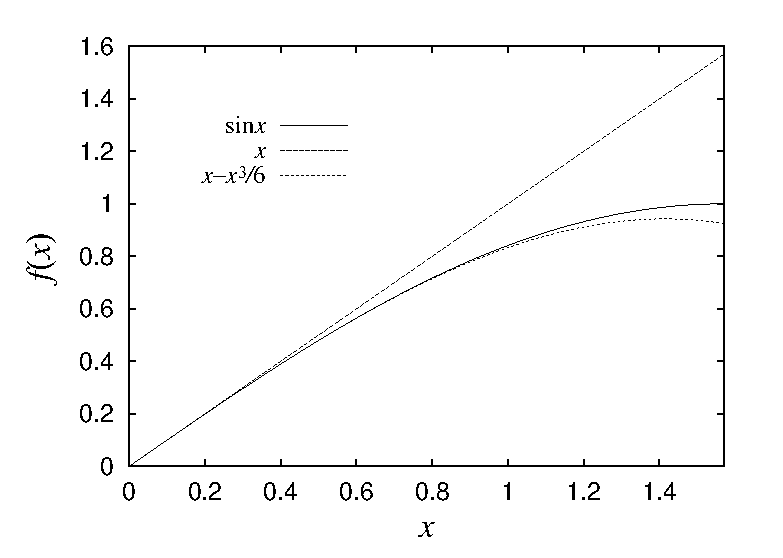
\includegraphics[width=.5\linewidth]{fig/pi_tailor.eps}
  \end{center}
  \caption{
    $\sin x$のテイラー展開の様子。1次関数で近似しても
    $x$が小さい範囲ならそれなりに、3次まで取ればかなりの
    範囲で元の関数を再現していることが分かるだろう。
  }
\end{figure}

%-----------------------------------------------------------------------
\newpage
\section{第二回 微分方程式の解法}
%-----------------------------------------------------------------------

\subsection{目的}
変数分離法、定数変化法など、代表的な線形偏微分方程式の解法を学ぶ。
特に、線形性について学び、変数分離法により微分方程式が
固有値問題となることを理解する。

\subsection{解答}

\ans{6}{1}
$$\frac{\diff y}{\diff x} = \frac{\ln x}{y} $$
変数分離型であるから、$y$を左辺に移項して
$x$で積分すればよい。
$y$の積分は問題ないであろうが、
$x$の積分は$\ln x$を含むため、部分積分が必要となる。
積分を実行すると、
\begin{equation}
  \frac{y^2}{2} = x \ln x - x + C
\end{equation}
を得る。

\ans{6}{2}
$$\frac{\diff y}{\diff x} + y= 2 \sin x $$
定数変化法を用いる。
まず、$2\sin x$を無視すると
\begin{equation}
  \frac{\diff y}{\diff x} + y= 0
\end{equation}
である。この微分方程式の一般解は
$$
  y = C \e^{-x}
$$
である。この事実から、もとの微分方程式の解を
$$
  y = C(x) \e^{-x}
$$
の形に仮定する。微分方程式に代入すると$C(x)$が満たすべき
微分方程式、
$$
  \frac{\diff C}{\diff x} =  2 \e^{x} \sin(x)
$$
が求める。これは容易に積分できて、
$$
  C(x) = \e^x (\sin x - \cos x) + C_2
$$
となる。$C_2$は新たな積分定数である。以上から
\begin{equation}
  y = \sin x - \cos x + C \e^{-x}
\end{equation}
と求まる(ただし積分定数$C_2$を$C$とおきなおした)。
微分方程式を解く場合、解の形を仮定して代入し、
より易しい方程式に落とす方法が良く取られる。
この定数変化法はその一つである。

\ans{6}{3}
$$\frac{\diff^2 y}{\diff x^2} + 3 \frac{\diff y}{\diff x} + 2y = 0 $$
微分方程式が同次形であるため、問題を解くこと自体は簡単である。
$y = \exp(\lambda)$の形を仮定して代入すると、$\lambda$に関する
代数方程式、
\begin{equation}
  \lambda^2 + 3 \lambda + 2 = 0
\end{equation}
を得る。この方程式を{\bf 特性方程式(characteristic equation)}と呼ぶ。
この方程式の解は$\lambda = -1, -2$であるから、
$y$は独立な解$\e^{-x}$及び$\e^{-2x}$を持つ。
以上から一般解は
$$
  y = C_1 \e^{-x} + C_2 \e^{-2x}
$$
を得る。二階微分方程式であるから、独立な積分定数を二つ含むことに注意せよ。

\ans{7}{1}
まず、
$$\frac{\diff^2 y}{\diff x^2} + 4 \frac{\diff y}{\diff x} + 3y = 0$$
の一般解は、
$$
  y = C_1 \e^{-x} + C_2 \e^{-3x}
$$
である。境界条件$y(0) = 0$、$y'(0) = 1$より、
連立方程式、
\begin{eqnarray}
  C_1 + C_2 &=& 0 \\
  -C_1 -3 C_2 &=& 1
\end{eqnarray}
が求まる。この解は、
$C_1 = 1/2, C_2 = - 1/2$であるので、特解は
$$
  y = \frac{1}{2}(\e^{-x} - \e^{-3x})
$$
と求まる。これは一度値が増え、その後減衰していく振る舞いを示している。

\ans{7}{2}
$$
  \frac{\diff^2 y}{\diff x^2} + 2 \frac{\diff y}{\diff x} + 2y = 0
$$
同様に$y = \exp(\lambda)$と仮定して特性方程式の根を求めると
$\lambda = -1 \pm i$と、複素共役な根を持つことが分かる。
$\lambda$が複素数であってもやることは同じで、
一般解は、
$$
  y = e^{-x} \left(C_1 \e^{ix} + C_2 \e^{-ix} \right)
$$
と求まるから、$y(0) = 1$、$y'(0) = 0$より、
$C_1 = (1-i)/2, C_2 = (1+i)/2$と求まる。
$\e^{ix} = \cos x + i \sin x$に注意して
解に代入して整理すると、
$$
  y = e^{-x} \left( \cos x + \sin x \right)
$$
となる。これは振動しながら減衰する、減衰振動を表す。

この式でわかるように、実部が振幅の時間発展を、虚部が振動項を
表している。したがって、{\bf 実部が正であればその解は$x \rightarrow \infty$で発散する}。
これは線形安定性解析と呼ばれる解析で用いられる最も基本的な事実である。
特性方程式の根の実部が正であるか負であるかは、解が
安定であるか不安定であるかという事実とつながっている。

\ans{8}{1}
$$ \frac{\partial u}{\partial t} =  \kappa \frac{\partial^2 u}{\partial x^2} $$
解の形を$u(x,t) = X(x)T(t)$と仮定して代入しよう。
すると、
\begin{equation}
  X \frac{\diff T}{\diff t} = \kappa T \frac{\diff^2 X}{\diff x^2}
  \label{eq_bunri}
\end{equation}
となる。ここで{\bf 偏微分が常微分になったことに注意せよ}。
$X(x)$、$T(t)$はそれぞれ$x$のみ、$t$のみの関数であるから、
それぞれの変数による偏微分は常微分となる。
式(\ref{eq_bunri})を整理すると
\begin{equation}
  \frac{1}{T} \frac{\diff T}{\diff t} = \kappa  \frac{1}{X} \frac{\diff^2 X}{\diff x^2}
\end{equation}
となる。左辺は$t$のみ、右辺は$x$のみに依存するから、
これが恒等式となるためには、それぞれ定数でなければならない。
その定数を後の便利のために$\lambda$とおくと、
\begin{eqnarray}
  \frac{\diff T}{\diff t} &= & \lambda T \label{eq_lambda} \\
  \frac{\diff^2 X}{\diff x^2} &= & \frac{\lambda}{\kappa} X
\end{eqnarray}
となる。以上から、偏微分方程式が常微分方程式に
帰着された。あとは常微分方程式と同様に解けばよい。
これが偏微分方程式における変数分離法である。
なお先取りになるが、これらがそれぞれ
固有値問題になっていることに注意したい。

さて、$T(t)$、$X(x)$それぞれの解は
\begin{eqnarray}
  T(t) &=& \e^{\lambda t}\\
  X(t) &=& \e^{\alpha x}, \e^{- \alpha x}
\end{eqnarray}
である(ただし$\alpha \equiv \sqrt{\lambda/\kappa}$)。
以上から一般解は
$$
  u(x,t) = C_1 \exp{(\lambda t + \alpha x)} + C_2 \exp{(\lambda t - \alpha x)}
$$
となる。ここで、$\lambda$や$\alpha$の次元に注意したい。
すでに述べたように指数関数の肩に次元のある量が乗ってはならない。
したがって、$\alpha$が長さの逆数の次元$[L^{-1}]$を、$\lambda$が時間の逆数の次元$[T^{-1}]$を
持っているはずである。たとえば
式(\ref{eq_lambda})を見れば、$\lambda$が時間の逆数の次元を
持っていることが分かるであろう。また、
元の微分方程式から$\kappa$の次元が$[L^2 T^{-1}]$であることに注意すれば、
$\alpha$が$[L^{-1}]$の次元を持つことも分かる。

\ans{8}{2}
境界条件として、任意の$t$において$u(0,t) = u(\pi,t) = 0$が与えられている。
まず、$\lambda$の符号によって場合わけをしなくてはならない。
$\lambda>0$の場合、$\alpha$は正の実数であるから、
$C_1 = 0$、$C_2 = 0$でなくてはならない。
すなわち、解は$u(x,t)=0$という定数関数となる。
このような解を{\bf 自明な(trivial)}解と呼び、物理的には
興味が無い。

そこで$\lambda <0$の場合を考える。
$\alpha \equiv \sqrt{\lambda/\kappa}$であることから、
$\lambda = -\kappa k^2$と置く。すると
$\alpha = i k$となることから一般解を書き直すと、
$$
  u(x,t) = \e^{- \kappa k^2 t}
  \left(
  C_1 \e^{ikx} +
  C_2 \e^{-ikx}
  \right)
$$
$u(0,t) = 0$より、$C_1 = - C_2$である。
さらに$u(\pi,t) = 0$から、$k = n \quad (n = 1,2,\cdots)$でなければならない。
以上をまとめると、解として
$$u(x,t) = C \e^{- \kappa n^2 t} \sin(nx)$$
を得る。ただし$C_1 = - C_2 = \displaystyle\frac{C}{2i}$とした。
偏微分方程式の微分の階数に比べて、条件が少ないために
積分定数をすべて決められないことに注意しよう。
この方程式は熱伝導方程式と呼ばれ、Fourier級数解析の
発見のきっかけとなった。得られた解は、最初に熱を持っていた
棒が、両端で冷やされ、全体として冷却されていく過程を表している。
またこれは、フーリエ級数展開の一例となっている。
Fourierは熱伝導の問題を解くためにフーリエ級数展開を考案したのである。

\ans{9}{1}
定義により、$u_1$、$u_2$が方程式の
解であるとき、$au_1 + bu_2$が方程式の解となるか
確かめればよい。
$u_1$、$u_2$が方程式の解であるから、それぞれ
\begin{eqnarray}
  \frac{\partial u_1}{\partial t} +  \frac{\partial^3 u_1}{\partial x^3} + 6  \frac{\partial u_1}{\partial x}  &=& 0\\
  \frac{\partial u_2}{\partial t} +  \frac{\partial^3 u_2}{\partial x^3} + 6  \frac{\partial u_2}{\partial x}  &=& 0
\end{eqnarray}
を満たす。それぞれ$a$倍、$b$倍して辺々足せば、
\begin{equation}
  \frac{\partial (au_1+bu_2)}{\partial t} +  \frac{\partial^3 (au_1+bu_2)}{\partial x^3} + 6  \frac{\partial (au_1+bu_2)}{\partial x}  = 0
\end{equation}
から、$au_1+bu_2$も解となっていることが分かる。
これは、微分演算子が線形であるからである。

\ans{9}{2}
$u$を解として、$c$倍した解$cu$が解であるか確かめよう。
代入すると、
\begin{eqnarray}
  c \frac{\partial u}{\partial t} +  c\frac{\partial^3 u_1}{\partial x^3} + 6 c^2 u\frac{\partial u_1}{\partial x}  &=&
  c \underbrace{\left( \frac{\partial u}{\partial t} +  \frac{\partial^3 u_1}{\partial x^3} + 6 u \frac{\partial u_1}{\partial x} \right)}_{=0} + 6c(c-1)u \frac{\partial u_1}{\partial x} \\
  &=& 6c(c-1) u\frac{\partial u_1}{\partial x} \\
  &\ne& 0
\end{eqnarray}
であるので、線形でないことがわかる。
この方程式は、 Korteweg-de Vries (KdV)方程式と呼ばれ、
浅い水の波を表す重要な非線形方程式である。

\subsection{解説}

\subsubsection{微分方程式とは}

微分方程式とは、微分演算子が含まれるような方程式である。
その中でも微分する独立変数が一種類であるようなものを
{\bf 常微分方程式(ordinary differential equation)}、
独立変数が複数含まれるものを
{\bf 偏微分方程式(partial differential equation)}と呼ぶ。
これらの方程式を微分を含まない形に書き直すことが目的である。
微分方程式を解く方法には長い歴史があり、様々な手法があるが、
基本的に微分方程式は「解けたらラッキー」なのであり、
一般的には解けるどころか解が存在するかどうかも非自明なものがほとんどである。

偏微分を常微分と区別するために$\partial$という記号を用いる。
$\partial/\partial x$は、他の独立変数を定数だと思って$x$で微分することである。
物理で扱う現象はほとんど空間と時間が関係している。
さらに我々が住む世界は3次元であるから、物理的な現象はほとんど
4つの独立変数$x,y,z,t$で記述される。
したがって、基本的に物理で扱う微分方程式は偏微分方程式である。
偏微分方程式も基本的には常微分方程式と同様に解けばよいが、
いくつか注意事項がある。

まず、微分をひっくり返してはいけない。常微分においては
\begin{equation}
  \frac{1}{\displaystyle \left( \frac{\diff y}{\diff x} \right)} = \frac{\diff x}{\diff y}
\end{equation}
であったが、偏微分は他の変数の依存性があるためにこうはならない。
詳しくはヤコビアンについて調べること。
また、(本質的に同じことであるが)常微分においては
\begin{equation}
  \frac{\diff y}{\diff x} \diff x = \diff y
\end{equation}
であったが、
\begin{equation}
  \frac{\partial y}{\partial x} \partial x = \partial y
\end{equation}
などとしてはならない。これについても詳しくは
全微分について調べること。

\subsubsection{微分方程式の解法}

微分方程式においては解の形を仮定して、代入していく方法が良く取られる。
代表的なものに{\bf 変数分離法}及び{\bf 定数変化法}などがある。
物理数学においては、とりあえずその二つを知っていれば良い。

変数分離法とは、解を異なる変数が積の形で書けると仮定して解く方法である。
常微分方程式の場合、微分方程式が
\begin{equation}
  \frac{\diff y}{\diff x} = X(x) Y(y)
\end{equation}
と書けるものを{\bf 変数分離型}と呼ぶ。ただし$X(x)$、$Y(y)$は
それぞれ$x$のみ、$y$のみを含む関数である。
変数分離型の微分方程式は、$Y(y)$を左辺に移項して両辺
$x$で積分すればよい。すなわち、
\begin{eqnarray}
  \frac{1}{Y(y)}\frac{\diff y}{\diff x} &=& X(x) \\
  \int \frac{\diff y}{\diff x} \diff x \frac{1}{Y(y)}  &=& \int \diff x X(x) +C \\
  \int \diff y \frac{1}{Y(y)}  &=& \int \diff x X(x) + C
\end{eqnarray}
として解を得ることが出来る。$C$は積分定数である。
このように積分定数を含む解を${\bf 一般解}$と呼ぶ。
一般解は微分方程式の解全体を表しており、微分の回数だけ
積分定数を含む。さらに初期条件や境界条件を考えると積分定数の値が確定し、
解が具体的に求まる。このようにして求まった解を{\bf 特殊解}、もしくは
{\bf 特解}と呼び、物理数学においては特解を求めるのが主な目的となる。

偏微分方程式においても変数分離法が存在する。
関数$u$が二つの独立変数$x,t$に依存するとしよう。
このとき、解の形を$u(x,t) = X(x)T(t)$の形に仮定して
微分方程式に代入し、常微分方程式の固有値問題に帰着させる方法である。
具体例を見たほうが早いと思うので、詳しくは解答を参照せよ。

定数変化法とは、
\begin{equation}
  \frac{\diff y}{\diff x} + y = f(x)
\end{equation}
のような形をしているとき、まず$f(x) = 0$とおいて
解を求め、積分定数$C$を$x$に依存するとして
もう一度代入して解を求める方法である。
これも解答を参照せよ。

微分方程式の一般解は積分定数という任意定数を含む。
しかし、物理で扱う問題では微分方程式のほかに条件がつく。
たとえば熱伝導の問題を解く場合は、境界での温度を指定する
必要があるだろう。物体の運動を扱う場合は、初期位置や初期速度を
与える必要がある。これらの条件を{\bf 境界条件 (boundary condition)}、
境界条件を満たす解を求める問題を{\bf 境界値問題 (boundary value problem)}と呼ぶ。
特に、$x=0$における値$y(0)$やその微分の値$y'(0)$を与える問題を
初期値問題と呼ぶ。
基本的には、まず一般解を求め、境界条件を満たすように積分定数を決めればよい。

\subsubsection{線形性}

微分方程式が一般には解くことが難しいことをすでに述べた。
しかし、線形微分方程式は解くことが可能である。
{\bf 線形(linear)}であるとは、{\bf 演算子 (operator)}$\cal L$と、{\bf 被演算子(operand)}$x,y$の
間に、$a$、$b$を定数として
\begin{equation}
  {\cal L} (a x + by) = a {\cal L}x +b {\cal L}y
\end{equation}
が成り立つことである。たとえば、演算子を行列、被演算子を
ベクトルだと思えば線形性が成り立つ(行列が線形代数と呼ばれる所以である)。
演算子として微分や積分、被演算子として関数だと思っても良い。

$y$が$x$にのみ依存するとする。
微分方程式が$y$、その微分(何階でも良い)、さらに$x$の関数の線形結合のみを含む場合、
その微分方程式を{\bf 線形微分方程式 (liner differential equation)}と呼ぶ(この微分方程式が線形性の定義を満たすことを確認せよ)。
特に$x$の関数を含まないものを{\bf 同次方程式(homogeneous linear equation)}と呼ぶ。
物理において線形微分方程式は非常に重要である。

同次方程式は、基本的に解を$\exp (\lambda x)$の形に仮定して解く。
これは、{\bf 指数関数が微分演算子の固有関数であるからである}。
{\bf 演算子 (operator)}と、{\bf 固有関数 (eigen function)}あるいは
{\bf 固有ベクトル (eigen vector)}について考えるのは、
解析の問題を代数に落とすためである。この事実は今後何度も強調されるであろう。

\yodan{余談コラム1}{%
  解析学(analysis)とは、微分、積分を代表とする
  極限操作を扱う学問である。それに対して代数学(algebra)とは、群論に代表されるように
  足し算や掛け算といった演算が定義された代数系が持つ構造を
  扱う学問である。群論や代数構造などというと難しく聞こえるかもしれないが、
  物理で扱う代数とは要するに「四則演算しか無い世界」のことなので、
  微分や積分が含まれる解析よりも計算が易しい。
  微分も積分も行列も、固有値問題を考える限り
  「線形代数」というひとくくりで考えることができてしまう。
  抽象的であればあるほど理解は難しくなるが、その分だけ適用範囲が広がり、強力な手法となる。
}

%-----------------------------------------------------------------------
\newpage
\section{第三回 基底と固有値問題}
%-----------------------------------------------------------------------

\subsection{目的}
ベクトル空間においても、関数空間においても、内積を定義すれば
線形空間として統一的に理解できることを学ぶ。
特に、直交基底による展開という概念に慣れる。

\subsection{解答}

\ans{10}{1}
固有値を$\lambda$とすると、特性方程式は
\begin{equation}
  \lambda^2 - 2 \lambda -3 = 0
\end{equation}
である。したがって、$\lambda = -1,3$を得る。
対応する規格化された固有ベクトルは、それぞれ
\begin{equation}
  {\bf e}_1 =
  \frac{1}{\sqrt{2}}
  \left(
  \begin{array}{c}
      1 \\ 1
    \end{array}
  \right)
  ,
  {\bf e}_2 =
  \frac{1}{\sqrt{2}}
  \left(
  \begin{array}{c}
      1 \\ -1
    \end{array}
  \right)
\end{equation}
である。この二つが直交していることは、内積が$0$であることから明らかである。
したがって、この二つのベクトルは正規直交基底である。

\ans{10}{2}
$\lambda_1 = -1$、$\lambda_2 = 3$とし、
対応する固有ベクトルをそれぞれ${\bf e}_1$、${\bf e}_2$としよう。
あるベクトル${\bf a}$が
$$
  {\bf a} = c_1 {\bf e}_1 +c_2 {\bf e}_2
$$
と展開できたとすると、${\bf e}_i$の正規直交性から、
$$
  c_i = {\bf e}_i \cdot {\bf a}
$$
であるから、
\begin{eqnarray}
  c_1 &=& \frac{7}{\sqrt{2}}\\
  c_2 &=& -\frac{1}{\sqrt{2}}
\end{eqnarray}
と求まる。

\ans{11}{1}
$V(x)=0$であるから、単に微分方程式
\begin{equation}
  -\frac{\hbar^2}{2m} \frac{\diff^2}{\diff x^2} \psi = E \psi
\end{equation}
を解けばよい。
$\alpha = \sqrt{2mE}/\hbar$とすれば、
\begin{equation}
  \psi(x) = A \e^{i \alpha x} + B \e^{- i \alpha x}
\end{equation}
が一般解である。
$C_1 = A+B$,$C_2 = i(A-B)$と置きなおすと、
\begin{equation}
  \psi(x) = C_1 \cos{\alpha x} + C_2 \sin{\alpha x}
\end{equation}



\ans{11}{2}
「$-L/2<  x < L/2$の範囲で自由に運動する」とは、
$-L/2<  x < L/2$の範囲では$V(x)=0$であり、
両端において$\psi(-L/2) = \psi(L/2) = 0$ということである。
この条件から前問の$C_1$、$C_2$、$E$を決めればよい。

$\psi(L/2) = 0$より、
\begin{equation}
  C_1 \cos{(\alpha L/2)} + C_2 \sin{(\alpha L/2)} = 0  \label{eq_psi1}
\end{equation}

$\psi(-L/2) = 0$より、
\begin{equation}
  C_1 \cos{(-\alpha L/2)} + C_2 \sin{(-\alpha L/2)} = 0 \label{eq_psi2}
\end{equation}
$\cos(-\theta) = \cos(\theta)$、$\sin(-\theta) = -\sin(\theta)$に注意して
(\ref{eq_psi1})+(\ref{eq_psi2})、(\ref{eq_psi1})-(\ref{eq_psi2})を計算すると、
\begin{equation}
  \left\{
  \begin{array}{c}
    C_1 \cos{(\alpha L/2)} = 0 \\
    C_2 \sin{(\alpha L/2)} = 0
  \end{array}
  \right.
\end{equation}
$C_1$と$C_2$が同時に$0$となる解には興味が無いので、
$\cos{\alpha L/2} = 0 $かつ$C_2=0$、もしくは$\sin{\alpha L/2} = 0 $かつ$C_1=0$である。
したがって、
\begin{eqnarray}
  \frac{L \alpha }{2} &=& \frac{n\pi}{2} \qquad (n = 1,2,\cdots)\\
  \frac{L \sqrt{2mE}}{2\hbar} &=& \frac{n\pi}{2} \\
  E &=& \frac{n^2 \hbar^2 \pi^2}{2mL^2}
\end{eqnarray}
すなわち、エネルギーは離散的な値をとる。
さて、規格化条件から$(\psi,\psi) = 1$でなくてはならない\footnote{%
  自分自身との内積の平方根をノルム(norm)と呼ぶ。実際には、ノルムの方が
  一般的な概念で、ここではノルムを内積によって定義していると考えたほうが良い。
}。したがって、
\begin{eqnarray*}
  (\psi,\psi) &=& \int_{-L/2}^{L/2} \!\! \diff x \psi^2(x) \\
  &=&  C^2 \int_{-L/2}^{L/2} \!\! \diff x \cos^2{\alpha x} \\
  &=& C^2 \int_{-L/2}^{L/2} \!\! \diff x \frac{1+\cos 2\alpha x}{2} \\
  &=& C^2 \left[ \frac{x}{2} +  \frac{\sin 2 \alpha x}{4 \alpha} \right]_{-L/2}^{L/2} \\
  &=& \frac{C^2 L}{2} \\
  &=& 1
\end{eqnarray*}
したがって、$C = \sqrt{2/L}$である。$\sin$の場合も半角公式の符号が逆になるだけで同様である。

以上をまとめると、
\begin{equation}
  E = \frac{n^2 \hbar^2 \pi^2}{2mL^2} \quad , \quad
  \psi(x) =
  \left\{
  \begin{array}{cc}
    \sqrt{\frac{2}{L}} \cos (\alpha x) & \quad n = 1,3,5,\cdots \\
    \sqrt{\frac{2}{L}} \sin (\alpha x) & \quad n = 2,4,6,\cdots
  \end{array}
  \right.
\end{equation}
ただし、$\alpha \equiv \sqrt{2mE}/\hbar$

\ans{11}{3}
前問より、波動関数は自然数$n$により区別される。エネルギー順位を
下から数えて$n$番目の波動関数を$\psi_n$と表そう。
異なるエネルギー固有値に対応する波動関数が直交するとは、
\begin{equation}
  (\psi_i,\psi_j) = \delta_{ij}
\end{equation}
が成り立つことであり、これを示せばよい。

まず、$n$が奇数の時には$\psi(x)$は偶関数、$n$が偶数の時には奇関数となるから、
$n$の偶奇が異なる波動関数の内積は$0$である(偶関数と奇関数を掛け算すると奇関数となり、
奇関数は原点に対して対称な範囲で積分すると$0$となるから)。
そこで、$n$が両方偶数、奇数の場合を考えればよい。

まず、$n$が両方奇数の場合、波動関数は
\begin{equation}
  \psi_n = \sqrt{\frac{2}{L}} \cos \alpha_n x
\end{equation}
とかける($\alpha_n = n \pi/L$)。
まず、$i \neq j$の時には、三角関数の和積の公式から、
\begin{eqnarray*}
  (\psi_i,\psi_j)& =& \frac{2}{L} \int_{-L/2}^{L/2} \!\!\! \diff x  \cos{(\alpha_i x)}  \cos{(\alpha_j x)}  \\
  &=& \frac{1}{L} \int_{-L/2}^{L/2} \!\!\! \diff x \left( \cos{((\alpha_i+\alpha_j) x)}  + \cos{((\alpha_i-\alpha_j) x)} \right)\\
  &=& 0
\end{eqnarray*}

次に、$i = j$の時には、三角関数の半角の公式から、
\begin{eqnarray*}
  (\psi_i,\psi_i)& =& \frac{2}{L} \int_{-L/2}^{L/2} \!\!\! \diff x  \cos^2{(\alpha_i x)}  \\
  &=& \frac{1}{L} \int_{-L/2}^{L/2} \!\!\! \diff x \left(
  1 +  \cos{(2\alpha_i x)}
  \right) \\
  &=& 1
\end{eqnarray*}
$n$が両方偶数の場合も同様である。
以上から、$(\psi_i,\psi_j) = \delta_{ij}$が示された。

\ans{12}{1}
微分方程式をあらわに書けば、
$$
  -\frac{\hbar^2}{2m} \frac{\diff^2}{\diff x^2} \psi  + \frac{m \omega^2 x^2}{2} \psi = E \psi
$$
となる。
計算を始める前に、$a$と$E$は$\psi$が解である条件から、
$N_0$は規格化条件から求まるということに気がついておきたい。

$$
  \frac{\diff^2}{\diff x^2} \psi_0 = (a^4x^2-a^2) \psi_0
$$
であるから、これを微分方程式に代入すると、
$$
  -\frac{\hbar^2}{2m} (a^4 x^2 -a^2)  + \frac{m \omega^2 x^2}{2} - E = 0
$$
$x$について整理すると、
$$
  \left( -\frac{\hbar^2 a^4}{2m}  + \frac{m \omega^2 }{2} \right)x^2 +
  \left( \frac{\hbar^2a^2}{2m} -E \right) = 0
$$
を得る。これが$x$に関して恒等式でなくてはならないから、
\begin{eqnarray*}
  a &=& \sqrt{\frac{m\omega}{\hbar}} \\
  E &=& \frac{1}{2} \hbar \omega
\end{eqnarray*}
と求まる。振幅$N_0$は、規格化条件$(\psi,\psi)=1$、すなわち
$$
  N_0^2 \int_{-\infty}^{\infty} \!\!\! \diff x  \exp(-a^2 x^2) = 1
$$
より、
$$
  N_0 = \sqrt{\frac{a}{\sqrt{\pi}}}
$$
と求まる。

\ans{12}{2}
$ax \rightarrow \xi$という変数変換を施すと、
$\displaystyle \frac{\diff}{\diff x} = a \displaystyle\frac{\diff}{\diff \xi}$であるから、
元の微分方程式は、
$$
  -\frac{\hbar^2 a^2}{2m} \frac{\diff^2}{\diff \xi^2} \psi +
  \left(
  \frac{m \omega^2}{2a^2} \xi^2 -E
  \right) \psi = 0
$$
となる。ここで、$a^2 = m\omega/\hbar$であることから代入して整理すると、
\begin{equation}
  - \psi'' + (\xi^2 - \frac{2E}{\hbar \omega})\psi = 0 \label{eq_hermite}
\end{equation}
となる。この変数変換が無次元化に対応することに注意したい。
$a$が距離の逆数の次元を持っている。したがって、$ax$は無次元量である。
一般に物理で出てくる微分方程式は無次元化すると式が簡単になる。

$$
  \psi(\xi) = N_n H_n(\xi) \exp(-\xi^2/2)
$$
であるから、
$$
  \psi'' = N_n( H_n'' - 2\xi H_n' + (\xi^2-1) H_n) \exp(-\xi^2/2)
$$
となる。これを(\ref{eq_hermite})式に代入すれば、
$$
  H_n'' - 2 \xi H_n +(\lambda -1)H_n = 0
$$
となる(ただし$\lambda \equiv 2E/\hbar \omega$)。
これが$H_n$が満たすべき微分方程式である。

\ans{12}{3}
$\psi_0$,$\psi_2$は偶関数、$\psi_1$は奇関数であるから、
$(\psi_0,\psi_1)=0$,$(\psi_1,\psi_2)=0$はすぐに分かる。
したがって非自明なのは$(\psi_0,\psi_2)$の計算である。
規格化定数を無視すると、
\begin{eqnarray*}
  (\psi_0,\psi_2) &=& \int_{-\infty}^{\infty}\!\!\! \diff x (4x^2-2) \e^{-x^2} \\
  &=& \int_{-\infty}^{\infty}\!\!\! \diff x  \left(
  -2x (\e^{-x^2})' - 2 \e^{-x^2} \right) \\
  &=& \int_{-\infty}^{\infty}\!\!\! \diff x  \left( 2\e^{-x^2} - 2 \e^{-x^2} \right)\\
  &=& 0
\end{eqnarray*}
ただし、途中で部分積分を行い、$x=\pm \infty$において$x \e^{-x^2} = 0$を用いた。
同様な計算で、$(\psi_n,\psi_n) = 1$も分かるが、計算は省略する。

\subsection{解説}

\subsubsection{線形代数と固有値問題}

線形偏微分方程式が、変数分離により常微分方程式に、さらに
固有値問題に落ちることを見てきた。そこで線形代数の固有値問題を復習しておこう。
行列$A$とベクトル${\bf x}$について、$A {\bf x} = \lambda {\bf x}$が
成り立つとき、${\bf x}$を$A$の固有ベクトル、$\lambda$を固有値と呼ぶ。
$A {\bf x} = \lambda {\bf x}$であることから、
\begin{equation}
  (A - \lambda I) {\bf x} = 0
\end{equation}
である(ただし$I$は単位行列)。
${\bf x} \ne 0$のベクトルが存在するためには行列$B = A - \lambda I$の
逆行列が存在してはいけない。したがって、$B$の行列式が$0$でなくてはならないことから
固有値$\lambda$の満たすべき方程式は
\begin{equation}
  |A - \lambda I|=0
\end{equation}
である。ただし$|\cdots|$は行列式を表す。
この方程式を固有方程式、もしくは微分方程式の場合と同様に
{\bf 特性方程式 (characteristic equation)}と呼ぶ。

また、行列のうち、$A=A^*$を満たすものをエルミート行列と呼ぶ。
$A$の要素がすべて実数である場合、エルミート行列は実対称行列となる。
エルミート行列の固有値は必ず実数である。また、相異なる固有値に属する固有ベクトル
同士は直交している。物理で出てくる演算子を行列表示すると
エルミート行列であることがほとんどなので、この事実は非常に重要である。

\subsubsection{固有ベクトルによる展開}

何か適当な空間を考える。たとえば$3$次元空間を考えよう。
このとき、次の3つのベクトル
\begin{equation}
  {\bf e}_1 =
  \left(
  \begin{array}{c}
      1 \\ 0 \\ 0
    \end{array}
  \right)
  \quad
  {\bf e}_2 =
  \left(
  \begin{array}{c}
      0 \\ 1 \\ 0
    \end{array}
  \right)
  \quad
  {\bf e}_3 =
  \left(
  \begin{array}{c}
      0 \\ 0 \\ 1
    \end{array}
  \right)
\end{equation}
は、これらの線形結合で$3$次元空間のすべてのベクトルを表現できる。
このとき、このベクトルは「$3$次元空間を張る\footnote{
  数学では「生成する」という表現を用いる。
}」と表現し、
このベクトルを{\bf 基底 (basis)}と呼ぶ。
基底の取り方は一意では無いが、独立な基底の数は決まっている(この場合は3)。
基底がお互いに直交している時、特に{\bf 直交基底 (orthogonal basis)}、
さらに自分自身との内積(絶対値)が$1$であるように選ばれた基底を
基底を{\bf 正規直行基底 (orthonormal basis)}と呼ぶ。

$n$次元エルミート行列$A$の
規格化された固有ベクトルを${\bf e}_i (i=1,2,\cdots,n)$とする。
これらは正規直交基底となるから、
任意の$n$次元ベクトル${\bf x}$は
\begin{equation}
  {\bf x} = c_1 {\bf e}_1 + c_2 {\bf e}_2 + \cdots + c_n {\bf e}_n
\end{equation}
と一意に分解することができる。
両辺に左から${\bf e}_i$をかけよう。すると正規直交性から、
\begin{equation}
  {\bf e}_i \cdot {\bf e}_j = \delta_{ij}
\end{equation}
であるから、
\begin{equation}
  {\bf e}_i \cdot {\bf x} = c_i
\end{equation}
である。すなわち、任意のベクトル${\bf x}$を固有ベクトルで展開したとき、
その展開係数は固有ベクトルと${\bf x}$との内積から求めることができる。

なぜこのように固有ベクトルで展開するのか。それは$A$と${\bf x}$との積を考える時に
便利だからである。${\bf e}_i$を固有値$\lambda_i$に対応する固有ベクトルとしよう。
固有ベクトルの定義から、$A{\bf e}_i = \lambda_i {\bf e}_i$であるから、
\begin{equation}
  A {\bf x} = c_1 \lambda_1 {\bf e}_1 + c_2 \lambda_2 {\bf e}_2 + \cdots + c_n \lambda_n {\bf e}_n
\end{equation}
である。行列とベクトルの掛け算を、単に$\lambda_i$というスカラー倍により計算できる。
ここでは$A$は行列であったが、一般には微分や積分でも良い。
本来微分などの解析的な計算が、固有関数で展開しておけば固有値の掛け算という
代数的な計算をするだけとなる。

\subsubsection{固有関数}

今まで演算子として行列を、被演算子としてベクトルを考えてきたが、
被演算子に関数を考えることもできる。
演算子$\cal{L}$に対して、$\cal{L} \psi = \lambda \psi$が成り立つ場合、
$\psi$を$\cal{L}$の固有関数、$\lambda$を固有値と呼ぶ。
$\cal{L}$は微分演算子や代数式、その線形結合などなどである。
特に物理においては、$\cal{L}$としてエネルギーに対応する
演算子を考えることが多く、この演算子を{\bf ハミルトニアン (Hamiltonian)}と呼び、
表記を$\cal H$とする。この場合、固有値がエネルギーをあらわす。


${\bf x}$と${\bf y}$をそれぞれ$n$次元のベクトルとすると、
ベクトルの内積$({\bf x},{\bf y})$は、
\begin{equation}
  ({\bf x},{\bf y}) \equiv {\bf x} \cdot {\bf y} = \sum_i^n x_i y_i
\end{equation}
と定義される。ただし$x_i$は${\bf x}$の第$i$成分である。
さらに、ベクトルの成分が複素数である場合には、
\begin{equation}
  ({\bf x},{\bf y}) \equiv \bar{{\bf x}} \cdot {\bf y} = \sum_i^n \bar{x_i} y_i
\end{equation}
と定義する。ただし$\bar{x_i}$は$x_i$の複素共役である。

さて、演算子に対する固有関数を考える限り、固有関数はベクトルのように扱うことができる。
ある二つの固有関数を$\psi(x),\phi(x)$としよう。値域は一般に複素数である。
これらの定義域を$a < x < b$とすると、
$\psi(x),\phi(x)$の内積$(\psi,\phi)$は、
\begin{equation}
  (\psi,\phi) = \int_{a}^{b} \!\!\! \diff x \psi^*(x) \phi(x)
\end{equation}
で定義される。ただし、$\psi^*(x)$は$\psi(x)$の複素共役である。
これは、関数が無限次元のベクトルだと思えば理解できるであろう。

\yodan{余談コラム2}{%
  普通、我々は3次元空間で定義されるベクトルが3次元ベクトルであると考える。
  しかし、数学では、3次元ベクトルで定義される空間が$3$次元空間であると考える。
  より正確に言えば、線形独立な3つのベクトルがあったとして、その線形結合で
  表すことができるベクトルの集合が3次元空間だと考えるのである。
  その意味で、空間とは要素に条件がある集合のことであり、
  その条件により名前がついている。
  たとえば、要素に和とスカラー倍が定義されている集合を
  ベクトル空間と呼ぶ。さらに内積が定義されているベクトル空間をヒルベルト空間と呼ぶ(これは不正確な表現だが)。
  ヒルベルト空間は物理で重要な役割を果たす。
}

\subsubsection{様々な基底}

ベクトル空間において、基底となるベクトルの取り方はいろいろあった。
たとえば2次元なら$(1,0),(0,1)$の二つにとっても良いし、
$(1/\sqrt{2},1/\sqrt{2}),(1/\sqrt{2},-1/\sqrt{2})$としても良い。
問題に応じて便利な基底を取ればよい。

同様に、関数空間においても様々な基底の取り方がある。
一番単純に、基底を$1,x,x^2,x^3,\cdots$ととることを考えよう。
これは$x=0$周りのテイラー展開を行ったことに対応する。
ただ、これらの基底は直交していないので使いづらいことが多い。
他に良く出てくる基底としては、ルジャンドル多項式(Legendre Polynomial) $P_n(x)$がある。
$P_n(x)$は$n$次の多項式で、
\begin{eqnarray*}
  P_0(x) &=& 1\\
  P_1(x) &=& x\\
  P_2(x) &=& \frac{1}{2}(3x^2-1)
\end{eqnarray*}
表される。$-1 < x < 1$の範囲で直交基底をなすことが分かる。
具体的には、
\begin{equation}
  (P_n,P_m) = \int_{-1}^{1} \!\!\!\diff x P_n(x) P_m(x)= \frac{2}{2n+1} \delta_{mn}
\end{equation}
が成り立つ(計算してみよ)。
他によく出てくる基底が、問題に出てくるエルミート多項式(Hermite Polynomial)である。
エルミートの多項式$H_n(x)$は、
\begin{eqnarray*}
  H_0(x) &=& 1\\
  H_1(x) &=& 2x\\
  H_2(x) &=& 4x^2-2
\end{eqnarray*}
である。これは$H_n(x) \exp(-x^2/2)$が$-\infty < x < \infty$の範囲で
直交基底をなす。
これらの多項式を陽に扱って計算をするのは大変であるが、それぞれが
ベクトルと同様に単なる基底だと思えば計算が非常に楽になる。


%-----------------------------------------------------------------------
\newpage
\section{第四回 フーリエ級数展開と超関数}
%-----------------------------------------------------------------------

\subsection{目的}
フーリエ級数展開が、直交基底による展開の特別な場合になっていることを理解する。
また、超関数が内積によって定義されることを学ぶ。

\subsection{解答}

\ans{13}{1}

絶対値がついているので$x=0$で微分不連続だが、それでも
すぐに偶関数だから$\cos$の成分しか出てこないということに気が付いて欲しい。
したがって$b_n = 0$である。

さて、
\begin{equation}
  a_n = \frac{1}{ \pi} \int_{-\pi}^{\pi} \!\!\! \diff x f(x) \sin nx
\end{equation}
であるから、

\begin{equation}
  a_0 = \frac{2}{\pi} \int_0^{\pi} x \diff x  = \pi
\end{equation}
ただし、$f(x)$の偶関数性を用いた。
$n\neq 0$の場合は、部分積分を用いれば
\begin{eqnarray}
  a_n &=& \frac{2}{\pi} \int_0^{\pi} x \cos nx \diff x \\
  &=& \frac{2}{\pi} \int_0^{\pi} x (\frac{1}{n}\sin nx)' \diff x  \\
  &=& \frac{2}{\pi} \left[ \frac{x}{n} \sin nx \right]_0^{\pi}
  - \frac{2}{n\pi} \int_0^{\pi} \sin nx \\
  &=& \frac{2}{n^2\pi} \left[\cos nx \right]_0^{\pi}\\
  &=& \frac{2 ((-1)^n -1)}{n^2\pi}
\end{eqnarray}
以上から、
\begin{eqnarray}
  f(x) = \frac{\pi}{2} + \frac{2}{\pi} \sum_{n=1}^\infty \frac{((-1)^n -1)}{n^2} \cos nx \\
  &=&
  \frac{\pi}{2} - \frac{4}{\pi} \sum_{m=0}^\infty \frac{\cos (2m+1)x}{(2m+1)^2} \\
\end{eqnarray}
$x=0$を代入すると、右辺、左辺共に$0$となり、一致する(はずである)。

\ans{13}{2}
前問と同様に奇関数であるから、$\sin$の成分しか出てこない。
したがって$a_n=0$である。
\begin{eqnarray}
  b_n &=& \frac{2}{\pi} \int_0^{\pi} \diff x  \sin nx\\
  &=& \frac{2}{\pi}  \left[ \frac{- \cos nx}{n}  \right]_0^\pi\\
  &=& \frac{2}{\pi} \frac{1 - (-1)^n}{n}
\end{eqnarray}
以上から、
\begin{equation}
  f(x) = \frac{2}{\pi} \sum_{n=1}^{\infty} \frac{1 - (-1)^n}{n} \sin nx
\end{equation}
さて、定義から$f(0) = 1$であるが、右辺の級数に$x=0$を代入すると$0$に
なってしまい、一致しない。
一般に、$f(x)$がある点$x_0$で不連続である場合には、
フーリエ級数は
\begin{equation}
  \lim_{\varepsilon \rightarrow 0} \frac{f(x_0 + |\varepsilon|) + f(x_0 - |\varepsilon|) }{2}
\end{equation}
すなわち、その不連続点における上側からの極限値と
下側からの極限値の平均値となる。
したがって、フーリエ級数展開、
\begin{equation}
  f(x) = \frac{a_0}{2} + \sum_{n=1}^\infty (a_n \cos nx + b_n \sin nx)
\end{equation}
は、厳密には不連続点で等号が成立しない。

\ans{14}{1}
複素フーリエ級数の和を、$n=0$と$n\le -1$、$n \ge 1$に分けることを考える。
\begin{eqnarray}
  f(x) &=& \sum_{n=-\infty}^{\infty} c_n \exp{(inx)}\\
  &=& \sum_{n=-\infty}^{\infty} c_n (\cos nx + i \sin nx)\\
  &=& c_0 + \sum_{n=1}^{\infty} c_n (\cos nx + i \sin nx)
  + \sum_{n=-1}^{-\infty} c_n (\cos nx + i \sin nx)\\
  &=& c_0 + \sum_{n=1}^{\infty} c_n (\cos nx + i \sin nx)
  + \sum_{n=1}^{\infty} c_{-n} (\cos nx - i \sin nx)\\
  &=& c_0 + \sum_{n=1}^{\infty} \left( (c_n+c_{-n}) \cos nx + i(c_n-c_{-n}) \sin nx  \right)
\end{eqnarray}
一方、フーリエ級数展開は、
\begin{equation}
  f(x) = \frac{a_0}{2} + \sum_{n=1}^{\infty} \left( a_n \cos nx + b_n \sin nx  \right)
\end{equation}
であるから、係数を比較して、
\begin{eqnarray}
  a_0 &=& 2 c_0 \\
  a_n &=& c_n + c_{-n} \\
  b_n &=& c_n - c_{-n}
\end{eqnarray}
より、$c_n$、$c_{-n}$について逆に解けば(\ref{eq_fourier_prefoctor})式の関係が得られる。

\ans{14}{2}

\begin{eqnarray}
  c_n &=& \frac{1}{2\pi} \int_{-\pi}^{\pi} \diff x \e^x \e^{-inx} \\
  &=& \frac{1}{2\pi} \int_{-\pi}^{\pi} \diff x \e^{(1-in)x} \\
  &=& \frac{1}{2\pi} \left[ \frac{\e^{(1-in)x}}{1-in}  \right]_{-\pi}^{\pi}\\
  &=& \frac{1}{2\pi} \left( \frac{\e^{(1-in)\pi} - \e^{(1-in)(-\pi) }}{1-in}  \right)\\
  &=& \frac{1}{2\pi} \left( \frac{ \e^\pi \e^{-in\pi} - \e^{-\pi} \e^{in\pi} }{1-in}  \right)\\
  &=& \frac{(-1)^n}{2\pi} \left( \frac{\e^{\pi} - \e^{-\pi} }{1-in}  \right)\\
  &=& \frac{(-1)^n}{\pi} \frac{\sinh \pi }{1-in}
\end{eqnarray}
以上から、
\begin{equation}
  f(x) = \sum_{n=-\infty}^{\infty} \frac{(-1)^n}{\pi} \frac{\sinh \pi }{1-in} \e^{inx}
\end{equation}
さて、$x=0$を代入すると、
\begin{eqnarray}
  f(0) &=& \sum_{n=-\infty}^{\infty} \frac{(-1)^n}{\pi} \frac{\sinh \pi }{1-in} \e^{inx}\\
  &=& \sum_{n=-\infty}^{\infty} \frac{(-1)^n}{\pi} \frac{(1+in) \sinh \pi }{1+n^2}\\
  &=& \frac{\sinh \pi}{\pi}\left( 1+  \sum_{n=1}^{\infty}\frac{(-1)^n(1+in)}{1+n^2}+\frac{(-1)^{-n}(1-in)}{1+n^2}  \right)\\
  &=& \frac{\sinh \pi}{\pi}\left( 1+  2 \sum_{n=1}^{\infty} \frac{(-1)^n}{1+n^2} \right)
\end{eqnarray}
さて、もともと$f(x)=\e^x$であったから、$f(0)=1$である。
以上から、
\begin{equation}
  \sum_{n=1}^{\infty} \frac{(-1)^n}{1+n^2} = \frac{1}{2} \left( \frac{\pi}{\sinh \pi} -1 \right)
\end{equation}

\ans{15}{1}
よくやる間違いは、$x = 0$なら$x \delta(x) = 0$、
$x \neq 0$なら$\delta(x) = 0$だから$x \delta(x) = 0$、
以上で証明終わり、とするものである。この証明は全くナンセンスである。
きちんとデルタ関数の定義に戻って
適当な関数$f(x)$との内積を考えなくてはいけない。

デルタ関数は内積でしか定義できないので、等価性を示す場合も内積の形で示す必要がある。
すなわち、内積ができる量$A$、$B$があったとき、
\begin{equation}
  (A,f(x)) = (B,f(x)) \quad \left( ^\forall f(x) \right)
\end{equation}
である場合に$A=B$と言うことができる\footnote{%
  ここで、内積の一意性を用いていることに注意。
}。

\begin{eqnarray}
  (x \delta(x), f(x) ) &= &\int_{-\infty}^\infty \!\!\! x \delta(x) f(x) \diff x \\
  &=& \int_{-\infty}^\infty \!\!\! \delta(x) g(x) \diff x \\
  &=& g(0) \\
  &=& 0 \\
  &=& (0, f(x))
\end{eqnarray}
ただし途中で$g(x) \equiv x f(x)$とおいた。
以上から$ x \delta(x)$はどのような(性質の良い)関数と内積をとっても$0$となる、すなわち、
\begin{equation}
  (x \delta(x), f(x)) = (0, f(x))
\end{equation}
であるから、$x \delta(x) = 0$と言う事ができる。

$ \delta(ax) = \delta(x)/|a|$の証明は以下の通り。
$a > 0 $のとき、
\begin{eqnarray}
  (\delta(ax),f(x)) &=& \int_{-\infty}^\infty \!\!\! \delta(ax) f(x) \diff x \\
  &=& \int_{-\infty}^\infty \!\!\! \delta(x) f(x/a) a \diff x\\
  &=& a f(0) \\
  &=& a \int_{-\infty}^\infty \!\!\! \delta(x) f(x) \diff x\\
  &=& (a \delta(x), f(x))
\end{eqnarray}
以上で、$a\delta(x) = \delta(ax)$が証明された。
$a<0$の場合は、積分区間が逆になることから負符号が出て、
あわせて$ \delta(ax) = \delta(x)/|a|$が結論される。

\ans{15}{2}
\begin{eqnarray}
  \left(  \frac{\diff \theta(x)}{\diff x} ,f(x) \right)
  &=& \int_{-\infty}^\infty \!\!\! \diff x \frac{\diff \theta(x)}{\diff x} f(x) \\
  &=&
  \left[
    \theta(x) f(x)
    \right]_{-\infty}^{\infty}
  - \int_{-\infty}^\infty \!\!\! \diff x \theta(x) f'(x)\\
  &=& - \int_{0}^\infty \!\!\! \diff xf'(x)\\
  &=& - f(\infty) + f(0)\\
  &=& \int_{-\infty}^\infty \!\!\! \diff x \delta(x) f(x)\\
  &=& (\delta(x), f(x))
\end{eqnarray}
以上から、
$$
  \displaystyle\frac{\diff \theta(x)}{\diff x} = \delta(x)
$$
が証明された。

\ans{15}{3}
デルタ関数の定義から、
\begin{eqnarray}
  c_n &=& \frac{1}{2\pi} \int_{-\pi}^{\pi} \!\!\! \diff x \delta(x) \e^{-inx} \\
  &=& \frac{1}{2\pi}
\end{eqnarray}
以上より形式的に、
\begin{equation}
  \delta(x) = \frac{1}{2\pi} \sum_{n=-\infty}^{\infty} \e^{inx}
\end{equation}
である。これはデルタ関数の級数表示である。デルタ関数にはいくつもの表示方法があるが、
それぞれ等価であるから計算に対して便利なものを場合に応じて使い分ければよい。

\subsection{解説}

\subsubsection{フーリエ級数展開}

$(-\pi \le x < \pi)$で定義されている関数$f(x)$を、
$$
  f(x) = \frac{a_0}{2} + \sum_{n=1}^\infty (a_n \cos nx + b_n \sin nx)
$$
の形に展開することをフーリエ級数展開という。
また、$a_n, b_n$をフーリエ係数と呼ぶ。

三角関数の直交性、
\begin{eqnarray}
  \int_{-\pi}^{\pi} \!\!\! \diff x \cos nx \cos mx &=& \pi \delta_{nm}
\end{eqnarray}
\begin{eqnarray}
  \int_{-\pi}^{\pi} \!\!\! \diff x \sin nx \sin mx &=& \pi \delta_{nm}
\end{eqnarray}
\begin{eqnarray}
  \int_{-\pi}^{\pi} \!\!\! \diff x \sin nx \cos mx &=& 0
\end{eqnarray}
より、フーリエ係数は
\begin{eqnarray}
  a_n = \frac{1}{ \pi} \int_{-\pi}^{\pi} \!\!\! \diff x \cos nx f(x)
\end{eqnarray}
\begin{eqnarray}
  b_n = \frac{1}{ \pi} \int_{-\pi}^{\pi} \!\!\! \diff x \sin nx f(x)
\end{eqnarray}
で求めることができる。たまにフーリエ級数展開の定義を
$$
  f(x) = \frac{a_0}{2\sqrt{\pi}} + \frac{1}{\sqrt{\pi}}\sum_{n=1}^\infty (a_n \cos nx + b_n \sin nx)
$$
として、フーリエ係数を
\begin{eqnarray}
  a_n = \frac{1}{ \sqrt{\pi}} \int_{-\pi}^{\pi} \!\!\! \diff x \cos nx f(x)
\end{eqnarray}
\begin{eqnarray}
  b_n = \frac{1}{\sqrt{\pi}} \int_{-\pi}^{\pi} \!\!\! \diff x \sin nx f(x)
\end{eqnarray}
とする教科書もあるが、これは
$\displaystyle \frac{1}{\sqrt{\pi}} \sin nx$、$\displaystyle \frac{1}{\sqrt{\pi}} \cos nx$が正規直交基底になるためであり、
実用上は前者がよく使われる。

\subsubsection{複素フーリエ級数展開}

オイラーの関係式
\begin{equation}
  \e^{i\theta} = \cos \theta + i \sin \theta
\end{equation}
を使えば、フーリエ級数展開の$\cos$と$\sin$を同時に扱うことができる。
すなわち、$(-\pi \le x < \pi)$で定義されている関数$f(x)$を、
$$
  f(x) = \sum_{-\infty}^{\infty} c_n \exp{(inx)}
$$
という形に展開する。

ここで、係数$c_n$は複素数であり、フーリエ級数における係数
$a_n$および$b_n$との関係は次の通りである。
\begin{eqnarray}
  \left\{
  \begin{array}{ccc}
    c_0    & = & \displaystyle\frac{a_0}{2}         \\
    c_n    & = & \displaystyle\frac{a_n - i b_n}{2} \\
    c_{-n} & = & \displaystyle\frac{a_n + i b_n}{2}
  \end{array}
  \right.
  \label{eq_fourier_prefoctor}
\end{eqnarray}

複素フーリエ級数の直交性は次のように表される。
\begin{equation}
  \int_{-\pi}^{\pi} \diff x (\e^{imx})^* \e^{inx} =
  \int_{-\pi}^{\pi} \diff x \e^{i(n-m)x} = 2\pi \delta_{mn}
\end{equation}
ただし$(\cdots)^*$は複素共役をあらわす。
この直交性を用いれば、
\begin{equation}
  c_n = \frac{1}{2\pi} \int_{-\pi}^{\pi} \diff x  f(x) (\e^{inx})^*
  = \int_{-\pi}^{\pi} \diff x  f(x) \e^{-inx}
\end{equation}
と係数を求めることができる。
$\e^{inx}$ではなく、$\e^{-inx}$をかけて積分をすることに注意したい。

以上のように、フーリエ級数展開と複素フーリエ級数展開は等価である。
しかし、こうやって指数関数であらわしてしまったほうが
三角関数を使うより計算は便利である。なぜなら
三角関数は微分や積分で$\sin$と$\cos$が入れ替わるが、
指数関数は指数関数のままで、肩に乗っている値を気にするだけでよいからだ。
また、複素フーリエ級数展開は、後に扱うフーリエ変換につながる。


\subsubsection{超関数}

次の積分で定義される関数$\delta(x)$を、ディラック(Dirac)のデルタ関数という。
$$
  \int_{-\infty}^{\infty} \!\!\! \diff x \delta(x) f(x) =
  \int_{-\varepsilon}^{\varepsilon} \!\!\! \diff x \delta(x) f(x) =
  f(0)
$$
ただし$\varepsilon$は任意の正数であり、関数$f(x)$は
$x = \pm \infty$で任意の$x$のべき乗よりも早く$0$に収束し、
さらに何回でも微分できるとする(このような関数を「性質の良い関数」と呼ぶ)。

この積分がデルタ関数と関数$f(x)$の内積、$(\delta,f)$になっていることに注意したい。
すなわち、{\bf デルタ関数とは、内積をとって初めて定義される関数}である\footnote{%
  デルタ関数には他にもいろいろ定義があるが、とりあえず積分(内積)によって定義される、
  と覚えておけば良い。
}。
このような関数を{\bf 超関数 (generalized function)}と呼ぶ\footnote{%
  distributionとも呼び、通常の関数functionと区別することがある。
  超関数の定義の仕方は一通りではない。それぞれが同じ超関数を定義しうるかなどは
  難しい問題だが、とりあえずここではこの定義で覚えておけば問題は無い。
}。

数学的にはだいぶ違う問題だが、微分などの演算子も、演算して初めて
意味を持つことに注意したい。
たとえば、$\displaystyle \frac{\diff}{\diff x} x$という「演算子」を考える。
演算子$A$、$B$の積 $AB$は、「最初に$B$を演算し、次に$A$を演算する」という意味である。
したがって、たとえば関数$f(x)$に先ほどの演算子を演算すると
\begin{equation}
  \frac{\diff}{\diff x} (x f(x)) = f(x) + x \frac{\diff f(x)}{\diff x}
\end{equation}
となる。したがって、元の演算子$\displaystyle \frac{\diff}{\diff x} x$と、
演算の順序を入れかえた$\displaystyle x \frac{\diff}{\diff x}$は一致しない。
先ほどの結果から、

\begin{equation}
  (\frac{\diff}{\diff x} x) f(x)  =  (1 + x \frac{\diff }{\diff x}) f(x)
\end{equation}
すなわち、演算子だけを見れば、
\begin{equation}
  \frac{\diff}{\diff x} x -   x \frac{\diff }{\diff x} =  1
\end{equation}
という関係が成り立つ。このような関係を{\bf 交換関係 (commutation relation)}と呼び、
代数学において重要な役割を果たす。
一般に、演算子の積$AB$と、順序を逆にした積$BA$の差$AB-BA$を$[A,B]$と
あらわす。
つまり
\begin{equation}
  [A,B] = AB - BA
\end{equation}
である。もし$[A,B]=0$である場合、すなわち演算子の順序を入れ替えても
結果が変わらない場合、「演算子$A$と$B$は交換する」と言う。
このような交換関係は、量子力学の定式化などで威力を発揮する。
$A$や$B$は、たとえば先ほどの例のように微分演算子でも良いし、行列でも良い(行列も一般には交換しない)。
抽象的で理解しづらかったら具体例で考えるようにしたい。
特に、「演算子は何かに演算して初めて意味を持つ」ということを思い出そう。
このような抽象化が代数の難しさであると同時に、代数学の強みでもある。
$A$が微分であろうと積分であろうと行列であろうと、もっと他の演算子であろうと、
交換関係という普遍的な代数構造を持つのである。

%-----------------------------------------------------------------------
\newpage
\section{第五回 フーリエ変換}
%-----------------------------------------------------------------------

\subsection{目的}
フーリエ変換の定義を覚え、フーリエ変換により、線形微分方程式が
代数方程式となることを理解する。さらに、逆フーリエ変換の実行には
複素積分が必要となることを理解する。

\subsection{解答}

\ans{16}{1}
積分の線形性より明らか。

\ans{16}{2}
フーリエ変換の定義より、
\begin{equation}
  \hat{f}(k) = \int_{-\infty}^{\infty} \!\!\! \diff x f(x) \e^{-ikx}
\end{equation}
部分積分を用いることで、
\begin{eqnarray}
  \hat{f}(k) &=& \int_{-\infty}^{\infty} \!\!\! \diff x f(x) \left( \frac{\e^{-ikx}}{-ik}\right)'\\
  &=&
  \left[
    f(x)  \frac{\e^{-ikx}}{-ik}
    \right]_{-\infty}^{\infty}
  + \frac{1}{ik}\int_{-\infty}^{\infty} \!\!\! \diff x f'(x) \e^{-ikx}\\
  &=& \frac{1}{ik}\int_{-\infty}^{\infty} \!\!\! \diff x f'(x) \e^{-ikx}
\end{eqnarray}
以上より、
\begin{equation}
  (ik) \hat{f}(k) = {\cal F}[f'(x)]
\end{equation}
以後、同様に繰り返すことで、
\begin{equation}
  (ik)^n \hat{f}(k) = {\cal F}[f^{(n)}(x)]
\end{equation}
を得る。

\ans{16}{3}
\begin{eqnarray}
  {\cal F}[f(x+a)] &=& \int_{-\infty}^{\infty} \!\!\! \diff x f(x+a) \e^{-ikx}\\
  &=& \int_{-\infty}^{\infty} \!\!\! \diff x f(x) \e^{-ik(x-a)}\\
  &=& \e^{ika} \int_{-\infty}^{\infty} \!\!\! \diff x f(x) \e^{-ikx}\\
  &=& e^{ika} \hat{f}(k)
\end{eqnarray}
ただし、途中で$x \rightarrow x-a$の変数変換を用いた。

\ans{16}{4}
フーリエ変換の定義より、
\begin{equation}
  \hat{f}(k) = \int_{-\infty}^{\infty} \!\!\! \diff x f(x) \e^{-ikx}
\end{equation}
両辺を$k$で形式的に微分すると、
\begin{eqnarray}
  \hat{f}'(k) &=& \int_{-\infty}^{\infty} \!\!\! \diff x (-ix) f(x) \e^{-ikx}\\
  &=& -i \int_{-\infty}^{\infty} \!\!\! x f(x) \e^{-ikx} \diff x\\
  &=& -i {\cal F}[x f(x)]
\end{eqnarray}
以上から、
\begin{equation}
  {\cal F}[x f(x)] = i \hat{f}'(k)
\end{equation}
同様に微分を繰り返せば、
\begin{equation}
  {\cal F}[x^n f(x)] = (i)^n \hat{f}^{(n)}(k)
\end{equation}
を得る。

\ans{16}{5}
フーリエ変換とたたみ込み積分の定義から、
\begin{eqnarray}
  {\cal F}[f*g] &=& \int_{-\infty}^{\infty} \diff x \e^{-ikx} \int_{-\infty}^{\infty} f(x-y)g(y)\diff y \\
  &=& \int_{-\infty}^{\infty} \diff y \e^{-iky} g(y) \int_{-\infty}^{\infty} \diff x \e^{-i(x-y)} f(x-y)\\
  &=& {\cal F}[g] {\cal F}[f]
\end{eqnarray}


\ans{17}{1}
\begin{eqnarray}
  \hat{f}(k) &=& \int_{-\infty}^{\infty} \!\!\! \diff x f(x) \e^{-ikx} \\
  &=& \int_{-a}^{a} \!\!\! \diff x \e^{-ikx} \\
  &=&
  \left[
    \frac{e^{ikx}}{-ik}
    \right]_{-a}^{a}\\
  &=& \frac{\e^{ika}-\e^{-ika}}{-ik}\\
  &=& \frac{2\sin ka}{k}
\end{eqnarray}

\ans{17}{2}
\begin{eqnarray}
  \hat{f}(k) &=& \int_{-\infty}^{\infty} \!\!\! \diff x f(x) \e^{-ikx} \\
  &=&
  \int_{-\infty}^{0} \!\!\! \diff x \e^{ax} \e^{-ikx}+
  \int_{0}^{\infty} \!\!\! \diff x \e^{-ax} \e^{-ikx}\\
  &=& \frac{1}{a-ik} + \frac{1}{a+ik} \\
  &=& \frac{2a}{a^2+k^2}
\end{eqnarray}

\ans{18}{1}
微分方程式全体をフーリエ変換すると、フーリエ変換の線形性より
\begin{equation}
  (ik)^2 \hat{y} - 2 (ik) \hat{y} = {\cal F}[\delta(x)]
\end{equation}
さて、デルタ関数のフーリエ変換は、
\begin{eqnarray}
  {\cal F}[\delta(x)] &=& \int_{-\infty}^{\infty} \!\!\! \diff x \delta(x) \e^{-ikx}\\
  &=& 1
\end{eqnarray}
以上より、
\begin{equation}
  (ik)^2 \hat{y} - 2 (ik) \hat{y} = 1
\end{equation}
整理すると、
\begin{equation}
  \hat{y}(k) = \frac{-1}{k^2+2ik}
\end{equation}
すなわち、{\bf フーリエ変換により線形微分方程式は代数方程式となる}。
これは後に学習するラプラス変換でも同様である。
ここで得られた$\hat{y}(k)$フーリエ逆変換すれば解$y(x)$が求められるが、
そのためには次の計算
\begin{equation}
  y(x) = \frac{1}{2 \pi} \int_{-\infty}^{\infty}\diff k \frac{-1}{k^2+2ik} \e^{ikx}
\end{equation}
を実行しなくてはならない。この積分には複素積分の知識が必要となる。

\ans{18}{2}
前問と同様にフーリエ変換を行うと、
\begin{equation}
  (ik)^2 \hat{y} - \hat{y} = {\cal F}[\e^{-ax^2}]
\end{equation}
となる。したがって、${\cal F}[\e^{-ax^2}]$を計算しなくてはいけない。
\begin{eqnarray}
  {\cal F}[\e^{-ax^2}] &=& \int_{-\infty}^{\infty}\diff x \e^{-ax^2} \e^{-ikx}\\
  &=& \int_{-\infty}^{\infty}\diff x \exp({-ax^2-ikx})\\
  &=& \int_{-\infty}^{\infty}\diff x \exp\left( -a \left(x+\frac{ik}{2}\right)^2 - \frac{k^2}{4a} \right)\\
  &=& \exp(-{\frac{k^2}{4a}})  \int_{-\infty}^{\infty}\diff x \exp\left( -a (x+\frac{ik}{2})^2 \right)\\
  &=& \sqrt{\frac{\pi}{a}} \exp(-{\frac{k^2}{4a}})
\end{eqnarray}
すなわち、{\bf ガウス分布のフーリエ変換はガウス分布となる}。
ただし、ガウス分布の広がり(分散)が逆になっていることに注意しよう。
すなわち、実空間でなだらかなガウス分布は、波数空間では狭い分布となる(逆もまたしかり)。
これはガウス分布だけでなく、フーリエ変換一般に言える性質である。

ちなみに、ここでフーリエ変換により微分方程式が代数方程式になったのは、
元の方程式が線形だったからである。
すなわち、{\bf 非線形微分方程式をフーリエ変換しても代数方程式にはならない}。
フーリエ変換はものの見方を変えているだけであって、
難しい問題は、変換しても難しいままとなるのである。

\subsection{解説}

問題で、
$$
  y''(x) - y(x) = \delta(x)
$$
の形の微分方程式を扱った。この解が求まると、一般の関数$f(x)$が含まれた
微分方程式
$$
  g''(x) - g(x) = f(x)
$$
の解を$y(x)$を使って表現できる。

まず、$y(x)$のフーリエ変換を考えると、
\begin{equation}
  {\cal F}[y] = -\frac{1}{k^2+1}
\end{equation}
また、$g(x)$のフーリエ変換は
\begin{equation}
  {\cal F}[g] = -\frac{1}{k^2+1} {\cal F}[f]
\end{equation}
したがって、
\begin{equation}
  {\cal F}[g] = {\cal F}[y] {\cal F}[f]
\end{equation}
左辺はたたみ込み積分のフーリエ変換として表現できるから、
\begin{equation}
  {\cal F}[g] = {\cal F}[y*f(x)]
\end{equation}
もとに戻すと、
\begin{equation}
  g(x) = \int_{-\infty}^{\infty}f(s) y(x-s)  \diff s
\end{equation}
以上より、一般の$f(x)$を含む微分方程式の解を得た。
あとはそれぞれの場合において$f(x)$を代入し、積分を実行すれば
$g(x)$を得ることができる。このように、デルタ関数は
たたみ込み積分と密接な関係を持つ。このことは後に学ぶ
ラプラス変換でより明らかとなる。


%-----------------------------------------------------------------------
\newpage
\section{第六回 複素積分とローラン展開}
%-----------------------------------------------------------------------

\subsection{目的}

複素関数の正則性および複素積分の基礎について学ぶ。
また、留数定理の準備として、ローラン展開について学ぶ。

\subsection{解答}

\ans{19}{1}

$z_0 = x_0 + i y_0$、
$x - x_0 = \Delta x$、
$y - y_0 = \Delta y$としよう。
$f(z)$の実部を$u(x,y)$、虚部を$v(x,y)$とすると、
$$
  \lim_{\Delta z \rightarrow 0} \frac{f(z+\Delta z) - f(z)}{\Delta z}
  =
  \lim_{\Delta z \rightarrow 0} \frac{u(x+\Delta z,y+\Delta y) - u(x,y)}{\Delta x + i \Delta y}
  + \lim_{\Delta z \rightarrow 0} i \frac{v(x+\Delta z,y+\Delta y) - v(x,y)}{\Delta x + i \Delta y}
$$
ここで、まず$y$軸をあわせて、$x$軸から近づく場合を考える。
すると、$\Delta y = 0$であるから、
\begin{eqnarray}
  \lim_{\Delta z \rightarrow 0} \frac{f(z+\Delta z) - f(z)}{\Delta z}
  &=&
  \lim_{\Delta x \rightarrow 0} \frac{u(x+\Delta x,y) - u(x,y)}{\Delta x}
  + \lim_{\Delta x \rightarrow 0} i \frac{v(x+\Delta x,y) - v(x,y)}{\Delta x}\\
  &=&
  \frac{\partial u}{\partial x} + i \frac{\partial v}{\partial x}
\end{eqnarray}
同様に、$\Delta x = 0$とすると、
\begin{eqnarray}
  \lim_{\Delta z \rightarrow 0} \frac{f(z+\Delta z) - f(z)}{\Delta z}
  &=&
  \lim_{\Delta y \rightarrow 0} \frac{u(x,y+\Delta y) - u(x,y)}{i\Delta y}
  + \lim_{\Delta y \rightarrow 0} i \frac{v(x,y+\Delta y) - v(x,y)}{i\Delta y}\\
  &=&
  -i \frac{\partial u}{\partial y} + \frac{\partial v}{\partial y}
\end{eqnarray}
を得る。分母に$i$があることに注意。
これらが一致しなくてはならないのだから、実部と虚部を比較すると、
コーシー・リーマンの関係式、
$$
  \frac{\partial u}{\partial x} = \frac{\partial v}{\partial y},
  \frac{\partial u}{\partial y} = -\frac{\partial v}{\partial x}
$$
を得る。

\ans{19}{2}

$z = x+ iy$とし、$z^2$の実部と虚部を求めると、
\begin{eqnarray}
  z^2 &=& (x+iy)^2\\
  &=& x^2 - y^2 +  2ixy
\end{eqnarray}
したがって、$u = x^2 - y^2$、$v = 2xy$
である。
それぞれ$x$および$y$で偏微分すればコーシー・リーマンの関係式を満たすことがわかる。
一般に、実部や虚部、絶対値や複素共役など、あらわに複素数を操作する関数以外の関数、
すなわち実数関数の$x$をそのまま$z$で置き換えた関数はほぼ正則であり、
その実部と虚部はコーシー・リーマンの関係式を満たすと思ってよい。

\ans{19}{3}
前問と同様に
$z = x+ iy$とし、$z^2$の実部と虚部を求めると、
\begin{eqnarray}
  z\bar{z} &=& (x+iy)(x-iy)\\
  &=& x^2 + y^2
\end{eqnarray}
したがって、この関数はつねに実数値をとるので、
実部と虚部の関係式であるコーシー・リーマンの関係式は満たさない。
なお、$z \bar{z} = |z|^2$、すなわち$z$の絶対値であることにも注意しておこう。

\ans{20}{1}

$z = (1+i)t$とおけば、積分は$t$をパラメータとして、
$$
  \int z^2 \diff z = \int_0^1 (1+i)^3 t^2  \diff t
$$
とあらわすことができる($\diff z = (1+i) \diff t$に注意せよ)。
これは簡単に積分できて、
$$
  (1+i)^3 \int_0^1 t^2  \diff t = \frac{(1+i)^3}{3}
$$
すなわち、単に$z$を実数の場合と同様に
$$
  \int_0^{1+i} z^2 \diff z = \left[ \frac{z^3}{3}  \right]_0^{1+i}
$$
とするのと同じ結果が得られた。
{\bf これは今回考えた関数が積分範囲で正則であったからである。}
一般に、積分範囲で正則な複素関数は、実数と同様に積分でき、
その値は積分経路に依存しない(積分値は始点と終点のみに依存する)。

\ans{20}{2}
点$a$を中心とする半径$r$の円は、極座標を用いて
$z = a + r\e^{i\theta} ~(0 \le \theta < 2\pi)$とあらわすことができる。
$\diff z = ri \e^{i\theta} \diff \theta$に注意すると、
もとの積分は$\theta$をパラメータとして、
\begin{equation}
  \oint (z-a)^n \diff z = i r^{n+1} \int_0^{2\pi} \e^{i(n+1)\theta} \diff \theta
\end{equation}
と表せる。
ここで、$n = -1$の場合とそうでない場合を分けて考えると、
\begin{equation}
  \oint (z-a)^n \diff z =
  \left\{
  \begin{array}{cccc}
    i r^{n+1} \left[ \displaystyle\frac{\e^{i(n+1)\theta}}{i(n+1)} \right]_0^{2\pi} & = & 0      & (n \neq -1) \\
    i \left[ \theta  \right]_0^{2\pi}                                               & = & 2\pi i & (n=-1)
  \end{array}
  \right.
\end{equation}
を得る。すなわち、$z^n$の形を特異点周りに周回積分した場合、
$1/z$以外はすべて$0$となる。これは重要な結果である。
後に述べるローラン展開において、適当な周回積分に寄与する項は
$c_{-1}$のみということを意味する。したがって、この項の値さえ
わかれば積分値が求められる。これも複素関数の正則性という
(関数にとって)厳しい条件からの帰結である。

\ans{21}{1}

$|z|<1$の場合、例に挙げられた展開で$-z$を代入すればよいから、
\begin{eqnarray}
  \frac{1}{z-1} &=& - \frac{1}{1-z}\\
  &=& -(1 + z + z^2 + \cdots + z^n + \cdots) \\
  &=& -\sum_{n=0}^{\infty} z^n
\end{eqnarray}

$|z|>1$の場合、$|1/z|<1$に注意すれば、
\begin{eqnarray}
  \frac{1}{z-1} &=& \frac{1}{z} \frac{1}{1 - 1/z}\\
  &=& z^{-1}
  \left(
  1 + z^{-1}+ z^{-2}+ \cdots
  \right)\\
  &=& \sum_{n=1}^{\infty} z^{-n}
\end{eqnarray}
すなわち、{\bf ローラン展開は同じ中心でも範囲によって係数が異なる}。
正確に言うと、範囲が新たな特異点をまたぐときに値が変わる。
これがなぜかは留数定理を学ぶときに明らかになるだろう。

\ans{21}{2}
まず、$f(z)$を部分分数分解すると、
\begin{equation}
  f(z) = \frac{1}{z(z-1)} = \frac{1}{z-1} - \frac{1}{z}
\end{equation}
あとは前問と同様に解くことができる。

\subsection{解説}

\subsubsection{正則性}
複素関数$f(z)$が、ある領域$D$のすべての点で微分可能であるとき、
$f(z)$は$D$において{\bf 正則 (holomorphic)}であるという。
複素関数$f(z)$がある点で微分可能であるためには、その実部と虚部に
コーシー・リーマンの関係式が成り立ってなくてはいけない。
この関係式をさらに$x$,$y$で偏微分してみよう。
\begin{eqnarray}
  \frac{\partial^2 u}{\partial x^2} &=& \frac{\partial^2 v}{\partial x \partial y}\\
  \frac{\partial^2 u}{\partial y^2} &=& - \frac{\partial^2 v}{\partial x \partial y}
\end{eqnarray}
すなわち、
\begin{equation}
  \Delta u = 0
\end{equation}
が成り立つことがわかる。ここで$\Delta \equiv \partial^2/\partial x^2 + \partial^2/\partial y^2$は
ラプラシアンである。
同様に、虚部である$v$についても
\begin{equation}
  \Delta v = 0
\end{equation}
が成り立つ。ラプラシアンを演算して0となる関数を
{\bf 調和関数 (Harmonic function)}であるという。
複素関数$f(z)= u(x,y) + i v(x,y)$が正則であるためには、
実部$u(x,y)$、虚部$v(x,y)$がそれぞれ調和関数でなくてはならない。
したがって、実数関数の微分可能性よりも厳しい条件が必要であり、
これが複素関数論の豊富な応用を生み出す。

複素関数が正則でないとは、たとえば$1/z$のように$\lim z \rightarrow 0$で無限大になってしまうものや、
$Re z$や$z \bar{z}$のように実部と虚部をあらわに操作する関数などがある。
しかし、本ゼミにおいては実積分のために複素積分を用いるのが目的なので
実用上は値が無限大になる点においては正則でないと覚えておけば良い。

\subsubsection{特異点}

関数$f(z)$が、点$a$では正則ではないが、その点の近傍に$f(z)$が正則であるような
点が存在するとき、$a$を$f(z)$の{\bf 特異点 (singular point)}と呼ぶ。
特に、$a$の任意の近傍に特異点が無い場合、$a$を孤立特異点と呼ぶ。
物理数学で扱われる特異点はほぼすべて孤立特異点である

点$a$が関数$f(z)$の孤立特異点である場合、そのまわりで、
\begin{equation}
  f(z) = \sum_{n=-\infty}^{\infty} c_n(z-a)^n
\end{equation}
と展開できる。これを{\bf ローラン(Laurent)展開}と言う。
このとき、$n\ge 0$の項、すなわち、
$\sum_{n=0}^{\infty} c_n(z-a)^n$は点$a$においても正則であるから、
$f(z)$の特異性は、残りの項
$\sum_{n=-\infty}^{-1} c_n(z-a)^n$
によると考えられる。この項をローラン展開の主要部と呼ぶ。

まず、主要部が無い場合は、点$a$を除きうる特異点と呼び、
$\lim_{z\rightarrow a} f(z)$の値を適当に再定義すれば
$f(z)$は$a$において正則となる。

主要部が無限項である場合、$a$を{\bf 真性特異点 (essential singularity)}と呼ぶ。
たとえば$\e^{1/z}$は、原点が真性特異点となる。

最後に主要部が有限項である場合、点$a$を{\bf 極 (pole)}と呼ぶ。
物理数学で扱うのは主にこの極である。特に、主要部の最高次数が$k$で
ある場合、$a$を$f(z)$の{\bf k位の極}と呼ぶ。


%-----------------------------------------------------------------------
\newpage
\section{第七回 留数定理とその応用}
%-----------------------------------------------------------------------

\subsection{目的}

留数定理を用いた複素積分と、その応用として実定積分の計算方法を学ぶ。

\subsection{解答}

\ans{22}{1}
$\e^{z}$は正則な関数であるから、公式で$f(z)=\e^z$、$a=-1$と置けばよい。
\begin{eqnarray}
  \frac{1}{2\pi i} \int_{|z|=2} \frac{\e^z}{z+1} &=& f(-1)\\
  &=& e^{-1}
\end{eqnarray}
すなわち、
\begin{equation}
  \int_{|z|=2} \frac{\e^z}{z+1} = 2\pi i e^{-1}
\end{equation}
ここで、積分路が囲む範囲$|z|<2$に、特異点$z=-1$が含まれることに注意しよう。
積分路が特異点を囲まなければ関数$\e^z/(z+1)$は正則となるので
周回積分は$0$である。

\ans{22}{2}
まず、部分分数分解を行う。
\begin{equation}
  \frac{z}{z^2+1} = \frac{1}{2} \left( \frac{1}{z+i} + \frac{1}{z-i} \right)
\end{equation}
コーシーの積分定理から、
\begin{eqnarray}
  \int_{|z|=2} \frac{1}{z+i} \diff z & =& 2 \pi i \\
  \int_{|z|=2} \frac{1}{z-i} \diff z & =& 2 \pi i \\
\end{eqnarray}
であるから、
\begin{equation}
  \int_{|z|=2} \frac{1}{z^2+1} = \frac{2\pi i + 2\pi i}{2} = 2 \pi i
\end{equation}

\ans{23}{1}
$f(z) = \e^{3z}$とおけば、コーシーの積分公式より、
\begin{equation}
  \frac{1}{2\pi i} \int_{|z|=3} \frac{f(z)}{(z-2)^2} = f'(2) = 3\e^{6}
\end{equation}
以上から、
\begin{equation}
  \int_{|z|=3} \frac{\e^{3z}}{(z-2)^2} = 6 \pi i \e^{6}
\end{equation}

\ans{23}{2}
まず注意したいのは、関数$\displaystyle \frac{1}{z^2(z-3)}$は
特異点として$z=0,3$を持つが、積分範囲$|z|=1$の中にあるのは$z=0$のみである。
したがって、関数$1/(z-3)$は積分領域で正則であるから、
$f(z) = 1/(z-3)$と置けば、
\begin{equation}
  \frac{1}{2\pi i} \int_{|z|=1} \frac{f(z)}{z^2} = f'(0) = - \frac{1}{9}
\end{equation}
したがって、
\begin{equation}
  \int_{|z|=1} \frac{1}{z^2(z-3)} =- \frac{2 \pi i}{9}
\end{equation}
このように、特異点のうち積分に寄与するのは、閉曲線の内部にあるもののみである。
これは、$|z|<3$と、$|z|>3$の二つの範囲で$\displaystyle \frac{1}{z^2(z-3)}$をローラン展開すればより明確に理解できよう。


\ans{24}{1}
まず、$\e^{iz}$は(無限遠を除いた)すべての領域で正則であることに注意しよう。
したがって特異点は$z = \pm i a$である。
部分分数分解すると、
\begin{equation}
  \frac{\e^{iz}}{z^2+a^2} = \frac{\e^{iz}}{2ia}
  \left(
  \frac{1}{z-ia} - \frac{1}{z+ia}
  \right)
\end{equation}
となる。
$z=ia$の周りで周回積分すると、
\begin{equation}
  \frac{1}{2\pi i} \int_{|z-ia|=\sigma} \frac{\e^{iz}}{2ia}
  \left(
  \frac{1}{z-ia} - \frac{1}{z+ia}
  \right)
  = \frac{\e^{-a}}{2ia}
\end{equation}
以上から、
\begin{equation}
  \mbox{Res} f(ia) = \frac{\e^{-a}}{2ia}
\end{equation}
同様に、$z=-ia$の周りで周回積分すれば、
\begin{equation}
  \mbox{Res} f(-ia) = - \frac{\e^{a}}{2ia}
\end{equation}
を得る。

{\bf 別解}\\
留数とは、ローラン展開したときの係数の$c_{-1}$そのものである。
したがって、$f(z)$が$a$を一位の極として持つなら、
\begin{equation}
  f(z) = c_{-1} (z-a)^{-1} + c_0 + c_1 (z-a) + c_2 (z-a)^2 + \cdots
\end{equation}
と展開されるはずである。
そこで、$f(z)(z-a)$をかけてから、極限$\lim z \rightarrow a$を考えると、
\begin{equation}
  \lim_{z \rightarrow a} f(z)(a-z) = c_{-1}
\end{equation}
となり、これは求める留数である。

この方法を問題に適用すると、
\begin{equation}
  \mbox{Res} f(ia) = \lim_{z \rightarrow ia} \left( (z-ia) \frac{\e^{iz}}{z^2+a^2} \right)
  = \frac{\e^{-a}}{2ia}
\end{equation}
\begin{equation}
  \mbox{Res} f(-ia) = \lim_{z \rightarrow -ia} \left( (z+ia) \frac{\e^{iz}}{z^2+a^2} \right)
  = -\frac{\e^{a}}{2ia}
\end{equation}
とすぐに求めることができる。
物理数学において複素積分は計算を簡単に行うための便法であるので、
複素積分自体もなるべく簡単に計算ができるように工夫したい。
そのためには典型的なパターンをいくつか覚える必要があるが、今回の例はその一つである。
他には$1/(1-z)$のテイラー展開を利用するものなどがある。

\ans{24}{2}
特異点は$\e^{i \pi /4}$、$\e^{i 3\pi /4}$、$\e^{-i \pi /4}$、$\e^{-i 3\pi /4}$の4つで、いずれも一位の極である。
部分分数展開しても良いが、前問の別解を使うほうが便利である。

$z = \e^{i \pi /4}$における留数は
\begin{equation}
  \mbox{Res} f(\e^{i \pi /4}) = \lim_{z \rightarrow \e^{i \pi /4}} \left( \frac{z-\e^{i \pi /4}}{z^4+1} \right)
  = \frac{\exp{(-3\pi i/4})}{4}
\end{equation}
ただし、$f(0)=g(0)=0$の時、
\begin{equation}
  \lim_{x\rightarrow 0} \frac{f(x)}{g(x)} = \frac{f'(x)}{g'(x)}
\end{equation}
を用いた(ロピタルの定理)。
他の留数も同様に求められる。

\ans{25}{1}
まず、$x^4+1$は偶関数であるから、
\begin{equation}
  \int_0^{\infty} \frac{1}{x^4+1} \diff x = \frac{1}{2} \int_{-\infty}^{\infty}  \frac{1}{x^4+1} \diff x
\end{equation}
として、以下の図のような積分路$C$を考える。
\begin{figure}[htbp]
  \begin{center}
    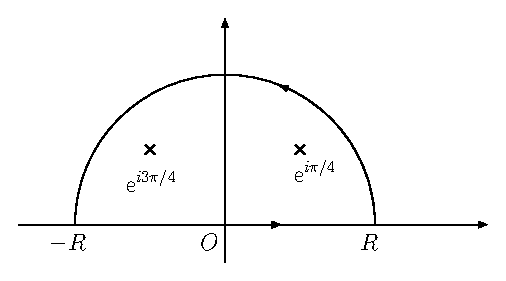
\includegraphics[width=.5\linewidth]{fig/z_int2.eps}
  \end{center}
  \caption{
    半円の積分路。$R$は無限大にする。
  }
  \label{fig_z_int2}
\end{figure}
ここで、$\lim R \rightarrow \infty$の極限で、半円の部分の積分の寄与は$0$となる(解説参照)。
したがって、
\begin{equation}
  \int_{-\infty}^{\infty} \frac{1}{x^4+1} \diff x = \lim_{R \rightarrow \infty} \int_C \frac{1}{z^4+1} \diff z
\end{equation}
ここで、積分路の内部にある特異点は$z = \e^{i\pi/4},\e^{i3\pi/4}$の二つであるから、
\begin{eqnarray}
  \int_C \frac{1}{z^4+1} \diff z &=& 2 \pi i \left( \mbox{Res} f(\e^{\pi i/4}) +\mbox{Res} f(\e^{3\pi i/4})  \right)\\
  &=& 2 \pi i \left(  \frac{\exp{(-3\pi i /4})}{4} + \frac{\exp{(-9 \pi i /4})}{4}  \right)\\
  &=& 2 \pi i \left(  \frac{\e^{\pi i/4}-\e^{- \pi i/4}}{4}  \right)\\
  &=& \pi \sin \frac{\pi}{4}
\end{eqnarray}
以上より、
\begin{equation}
  \int_0^{\infty} \frac{1}{x^4+1} \diff x = \frac{\pi}{2} \sin \frac{\pi}{4} = \frac{\pi}{2\sqrt{2}}
\end{equation}

\ans{25}{2}
$f(z) = \e^{ikz}/(z^2+1)$とし、以下の複素積分を考える。
\begin{equation}
  \int_C \frac{e^{ikz}}{z^2+1} \diff z
\end{equation}
まず、$f(z)$の上半面内の特異点は$z=i$のみであるので、
\begin{eqnarray}
  \int_C \frac{e^{ikz}}{z^2+1} \diff z &=& 2\pi i ~\mbox{Res} f(i)\\
  &=& 2\pi i \left( \frac{\e^{-k}}{2i} \right) \\
  &=& \pi \e^{-k}
\end{eqnarray}
以上から、
\begin{equation}
  \int_{-\infty}^{\infty} \frac{\cos kx}{x^2+1} \diff x =
  \mbox{Re} \int_C \frac{\e^{ikz}}{z^2+1} \diff z = \pi \e^{-k}
\end{equation}

\subsection{解説}

\subsubsection{コーシーの積分定理}

複素関数が微分可能であるとき、その実部と虚部には
強い制限(コーシー・リーマンの関係式)が課せられるのであった。
その帰結として、以下のコーシーの積分定理が成り立つ。

関数$f(z)$が領域$D$で正則であるとする。$C$は$D$内の単一閉曲線で、
$C$の内部が$D$の点のみであるとき、
\begin{equation}
  \int_C f(z) \diff z = 0
\end{equation}
が成り立つ。すなわち、{\bf 正則な関数を周回積分すると値が$0$となる}。
この積分定理と関数の正則性から、以下のコーシーの積分公式が導かれる。

関数$f(z)$は領域$D$であり、$C$は内部に領域$D$の点のみを持つ単一閉曲線である。
このとき、$C$内の点$a$について、以下の公式が成り立つ。
\begin{equation}
  f(a) = \frac{1}{2\pi i} \int_C \frac{f(z)}{z-a} \diff z \label{eq_cauchy1}
\end{equation}
これは、$C$の内部の任意の点$a$での値$f(a)$が$C$上の$f(z)$の値だけで決まる、
すなわち、{\bf 境界の値からその内部の値がすべて決まることを意味している}。
さらに以下の公式が成り立つ(これもコーシーの積分公式と呼ばれる)。
\begin{equation}
  f^{n}(a) = \frac{n!}{2\pi i} \int_C \frac{f(z)}{(z-a)^{n+1}} \diff z  \label{eq_cauchy2}
\end{equation}
すなわち、{\bf 積分の値が微分から求められる}。
これらの性質はすべて、複素関数が微分可能(正則)であるという条件が厳しいからである。
ここで、式(\ref{eq_cauchy2})は、式(\ref{eq_cauchy1})を形式的に左右$a$で微分した形に
なっていることに注意しよう。

さて、なぜコーシーの積分定理が成り立つか考えよう。
まず、$(z-a)^n$を$a$の周りに周回積分すると、その半径にかかわらず
\begin{eqnarray}
  \int_{|z-a|=r} (z-a)^n \diff z=
  \left\{
  \begin{array}{ccc}
     & 0      & (n \neq -1) \\
     & 2\pi i & (n = -1)
  \end{array}
  \right.
\end{eqnarray}
となるのであった。
また、$f(z)$が考えている領域で正則であるならば、
\begin{equation}
  f(z) = f(a) + f'(a) (z-a) + \frac{f''(a)(z-a)^2}{2} + \cdots
\end{equation}
と$a$の周りでテイラー展開できる。
したがって、
\begin{equation}
  \frac{f(z)}{z-a} = \frac{f(a)}{z-a} + f'(a) + \frac{f''(a)(z-a)}{2} + \cdots
\end{equation}
となるから\footnote{%
  これは$f(z)/(z-a)$の$a$におけるローラン展開である。
}、周回積分すれば、$1/(z-a)$の係数のみが残るので、
\begin{equation}
  \int_C \frac{f(z)}{z-a} \diff z = 2\pi i f(a)
\end{equation}
と、コーシーの積分公式を得た。
同様に$f(z)/(z-a)^{n+1}$の展開を考えることで公式(\ref{eq_cauchy2})も得ることができる。
記憶する便法として、$a$による形式的な微分をしても良いが、
ローラン展開をして$1/(z-a)$の係数を求めているのが本質であることを理解して欲しい。

\subsubsection{実定積分への応用}

複素積分は、実関数の定積分の値を求めるのに用いることができる。
複素積分を用いるのは、原始関数は求められないが、ある特別な区間においては定積分の値が求まる場合と、
原始関数が求められる場合でも複素積分を用いたほうが計算が簡単である場合がある。

物理数学において出てくる積分のパターンには、まず
\begin{equation}
  \int_{-\infty}^{\infty} \frac{f(x)}{g(x)} \diff x
\end{equation}
というタイプがある。ただし$f(x)$、$g(x)$はそれぞれ$m$次と$n$次の多項式であり、
$m\le n + 2$を満たすとする。さらに$g(x)=0$は実数解を持たないとする。

まず、前者の場合は、
積分路$C$を図\ref{fig_z_int2}のように半円型にとり、
複素積分
\begin{equation}
  \lim_{R \rightarrow \infty}\int_C \frac{f(z)}{g(z)} \diff z
\end{equation}
を考えるのが定石。ここで、円周の積分は半径$R$を無限大にすれば$0$となる。
それは、$f(z)$が$m$次、$g(z)$が$n$次の多項式であり、
$m\le n + 2$を満たすことから、$\lim |z| \rightarrow \infty$において
\begin{equation}
  \left| \frac{f(z)}{g(z)} \right| \leq \frac{1}{|z|^2}
\end{equation}
を満たす。
したがって、半径$R$の円周上$C_1$において
\begin{eqnarray}
  \int_{C_1} \frac{f(z)}{g(z)} \diff z &\leq& \int_{C_1} \left| \frac{f(z)}{g(z)} \right| \diff z \\
  &\leq& \int_{C_1}  \frac{1}{|z|^2} \diff z\\
  &= & \frac{1}{R}
\end{eqnarray}
以上から、$R \rightarrow \infty$の極限で、円周上の積分の寄与が$0$になるのである。
逆に、$|z| \rightarrow \infty$の極限に対して、$1/z^2$より早く$0$になる
複素関数でなければ、円周上の積分を$0$とおいてはいけない。

さて、円周の積分が$0$であるから、「実軸の積分」は「実軸を含む周回積分」と等しいことがわかる。
ここで、複素関数の周回積分は留数定理で簡単に値を求めることができる。
以上より実関数の定積分が複素積分により求められるのである。

複素積分を使った実定積分には、もう一つ
\begin{equation}
  \int_{-\infty}^{\infty} \frac{f(x)\cos(kx)}{g(x)} \diff x
\end{equation}
というパターンがある。ただし、$f(x)$と$g(x)$
それぞれ$m$次と$n$次の多項式であり、
$m\le n + 1$を満たすとする。さらに$g(x)=0$は実数解を持たないとする。

これは複素関数$F(z)$として、
\begin{equation}
  F(z) =  \frac{f(z) \e^{ikz}}{g(z)}
\end{equation}
を考えるのが定石である。
これについて複素積分を実行し、後で実部をとればよい。$\sin$の場合も同様に積分後に虚部を取る。

%-----------------------------------------------------------------------
\newpage
\section{第八回 フーリエ逆変換とジョルダンの補題}
%-----------------------------------------------------------------------

\subsection{目的}

フーリエ逆変換を行う際、複素積分の積分路をどのように取るべきかを学ぶ。

\subsection{解答}

\ans{26}{1}

フーリエ変換の定義より、
\begin{eqnarray}
  \hat{f}(k) &=& \int_{-\infty}^{\infty} f(x) \e^{-ikx} \diff x \\
  &=& \int_{-a}^{a} \e^{-ikx} \diff x \\
  &=& \left[ \frac{\e^{-ikx}}{-ik}  \right]_{-a}^a\\
  &=& \frac{1}{ik} \left( \e^{ika} - \e^{-ika} \right)
\end{eqnarray}

\begin{figure}[htbp]
  \begin{center}
    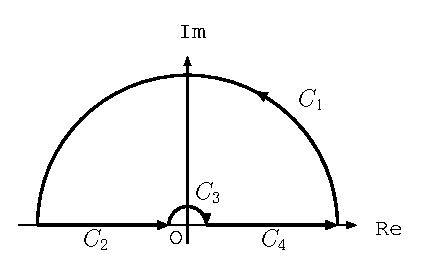
\includegraphics[width=.5\linewidth]{fig/jordan2.eps}
  \end{center}
  \caption{
    複素積分を行うための積分路。
    全体の積分路$C = C_1+C_2+C_3+C_4$は、積分路に特異点が無いから$0$。
    $(x+a)>0$であれば、十分大きな半径のとき$C_1=0$となる。
    また、$C_3$は、半径$0$の極限で$-\pi i $であり、
    求めたい積分は
    $
      \int_{-\infty}^{\infty} = \int_{C_2}+\int_{C_4} = -\int_{C_3}
    $
    から求まる。$(x+a)<0$の場合は下半面を回らなくてはいけない。
  }
  \label{fig_jordan2}
\end{figure}

\ans{26}{2}
逆フーリエ変換の定義から、
\begin{eqnarray}
  f(x) &=& \frac{1}{2\pi} \int_{-\infty}^{\infty} \hat{f}(k) \e^{ikx} \diff k \\
  &=& \frac{1}{2\pi i}\int_{-\infty}^{\infty} \left( \frac{\e^{i(x+a)k}}{k} - \frac{\e^{i(x-a)k}}{k} \right) \diff k
\end{eqnarray}
まず、第一項の積分を計算する。$x+a>0$の場合、
積分路$C$を図\ref{fig_jordan2}
$C = C_1 + C_2 + C_3 + C_4$のように取る。
$C$の中には極が無いから、
\begin{equation}
  \int_{C} \frac{\e^{i(x+a)z}}{z} \diff z = 0
\end{equation}
ジョルダンの補題より大きな半径を取れば$C_1= 0$である。
また、積分路$C_3$は、一位の極を時計回りに半分だけ回っているから
\begin{equation}
  \int_{C_3} \frac{\e^{i(x+a)z}}{z} \diff z = - \pi i
\end{equation}
である。以上から、
\begin{eqnarray}
  \int_{C_1+C_2+C_3+C_4} \frac{\e^{i(x+a)k}}{k} \diff k &= &0 \\
  \int_{C_2+C_4} \frac{\e^{i(x+a)k}}{k} \diff k - \pi i &= &0 \\
  \therefore \int_{-\infty}^{\infty} \frac{\e^{i(x+a)k}}{k} \diff k &=& \pi i
\end{eqnarray}
同様に、$x+a <0$の時には、
\begin{equation}
  \int_{C_2} \frac{\e^{i(x+a)z}}{z} \diff z = - \pi i
\end{equation}
となる。

まとめると、
\begin{equation}
  \int_{-\infty}^{\infty} \frac{\e^{i(x+a)k}}{k} \diff k =
  \left\{
  \begin{array}{cc}
    \pi i  & \quad (x > -a) \\
    -\pi i & \quad (x < -a)
  \end{array}
  \right.
\end{equation}
積分の第二項も同様に、
\begin{equation}
  \int_{-\infty}^{\infty} \frac{\e^{i(x-a)k}}{k} \diff k =
  \left\{
  \begin{array}{cc}
    \pi i  & \quad (x>a) \\
    -\pi i & \quad (x<a)
  \end{array}
  \right.
\end{equation}

以上をまとめると、
\begin{equation}
  f(x) = \left\{
  \begin{array}{cc}
    0 & \quad x < -a        \\
    1 & \quad -a \leq x < a \\
    0 & \quad a \leq x
  \end{array}
  \right.
\end{equation}
となり、確かに元の関数に一致する。

\ans{27}{1}

全体をフーリエ変換すると、
\begin{equation}
  (ik)^2 \hat{f} - \hat{f} = {\cal F}[\e^{-|x|}]
\end{equation}
ここで、
\begin{eqnarray}
  {\cal F}[\e^{-|x|}] & =&
  \int_{-\infty}^{\infty} \e^{-|x|} e^{-ikx} \diff x\\
  &=&
  \int_{-\infty}^{0} \e^{x} e^{-ikx} \diff x +
  \int_{0}^{\infty} \e^{-x} e^{-ikx} \diff x \\
  &=& \frac{1}{1-ik} + \frac{1}{1+ik}\\
  &=& \frac{2}{1+k^2}
\end{eqnarray}
以上から、
\begin{equation}
  \hat{f}(k) = - \frac{2}{(1+k^2)^2}
\end{equation}

\ans{27}{2}

逆フーリエ変換の定義より、
\begin{equation}
  f(x) = - \frac{1}{2\pi} \int_{-\infty}^{\infty}  \frac{\e^{ikx}}{(1+k^2)^2} \diff k
\end{equation}
$x>0$のとき、複素平面の上を通る半円を積分路とすると、
\begin{equation}
  \int_{-\infty}^{\infty}  \frac{\e^{ikx}}{(1+k^2)^2} \diff k
  = \int_C  \frac{\e^{ixz}}{(1+z^2)^2} \diff z
\end{equation}
このとき、積分路の中に、2位の極$z = i$があるから、
$F(z) = \displaystyle \frac{2 \e^{ixz}}{(z+i)^2}$とすれば、
\begin{eqnarray}
  \int_C  \frac{\e^{ixz}}{(1+z^2)^2} \diff z &=& \int_C  \frac{F(z)}{(z-i)^2} \diff z \\
  &=& 2 \pi i F'(i) \\
  &=& \frac{2\pi (1+x)}{2} \e^{-x}
\end{eqnarray}
すなわち、
\begin{equation}
  f(x) = - \frac{(1+x)}{2} \e^{-x}
\end{equation}

同様に、$x<0$のときは
\begin{equation}
  f(x) = - \frac{(1-x)}{2} \e^{x}
\end{equation}

まとめると、
\begin{equation}
  f(x) = - \frac{(1+|x|)}{2} \e^{-|x|}
\end{equation}

\ans{27}{3}

$x>0$のとき、
\begin{eqnarray}
  f(x) &=& -\frac{(1+x)}{2}e^{-x}\\
  \frac{\diff}{\diff x} f(x) &=& \frac{x}{2}e^{-x}\\
  \frac{\diff^2}{\diff x^2}  f(x) &=& \frac{(1-x)}{2}e^{-x}\\
\end{eqnarray}
以上から、
\begin{equation}
  \frac{\diff^2}{\diff x^2}  f(x) - f(x) = \e^{-x}
\end{equation}
$x<0$の場合も同様。

\subsection{解説}

関数$f(x)$のフーリエ変換$\hat{f}(k)$が存在するためには、積分
\begin{equation}
  \int_{-\infty}^{\infty} |f(x)|  \diff x
\end{equation}
が有限でなくてはならない。これを{\bf 絶対可積分}であるという。
フーリエ変換が可能である条件は、$f(x)$が区分的に滑らかで、
絶対可積分であることである。

さて、フーリエ逆変換は、以下の積分で与えられる。
\begin{equation}
  f(x) = \frac{1}{2\pi}\int_{-\infty}^{\infty} \hat{f}(k) \e^{ikx} \diff k
\end{equation}
さて、この積分を、複素積分を用いて
\begin{equation}
  f(x) = \frac{1}{2\pi} \int_{C} F(z) \e^{ixz} \diff z
\end{equation}
を用いて計算したい。このとき、積分路$C$をどのように決めるべきだろうか。
ただし、$|z| \rightarrow \infty$において$F(z) \rightarrow 0$であるとする。
複素積分においては、半円形の積分路が良く取られるが、
半円の半径$R$を十分大きくしたときに半円の積分の寄与が$0$になる必要がある。

まず、積分路を図\ref{fig_jordan}の$C_1$(複素平面の上半分の半円)のように取ることを考える。
$u,i$を実数とし、$z = u + iv$としよう。
\begin{equation}
  |\e^{ixz}| = |\e^{ixu - vx}| = \e^{- vx}
\end{equation}
であるから、$v \rightarrow \infty$、すなわち虚軸の上の方で
$\e^{ixz}$が$0$となるためには、$x>0$でなくてはならない。
逆に$x<0$の時には、$\displaystyle \lim_{\mbox{Im} z \rightarrow \infty} \e^{ixz} \rightarrow \infty$となるため、
積分路を$C_2$のように取らなくてはいけない。

以上をまとめて、
\begin{eqnarray}
  \lim_{R\rightarrow \infty}  \int_{C_1} F(z) \e^{iaz} \diff z &=& 0 \qquad (a>0)\\
  \lim_{R\rightarrow \infty}  \int_{C_2} F(z) \e^{iaz} \diff z &=& 0 \qquad (a<0)
\end{eqnarray}
を{\bf ジョルダンの補題}という。これはフーリエ逆変換を行う際、
積分路をどのように決めるべきかを考える上で重要である。

\begin{figure}[htbp]
  \begin{center}
    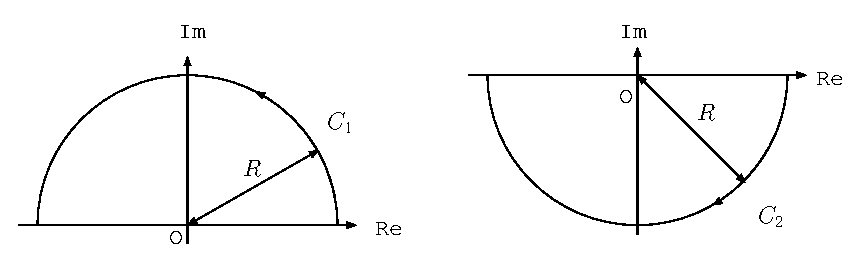
\includegraphics[width=.8\linewidth]{fig/jordan.eps}
  \end{center}
  \caption{
    ジョルダンの補題。$F(z)\e^{ikx}$の積分においては、
    $x$の値によって積分路を変える必要がある。
    $x>0$の場合は$C_1$(上半面)を、$x<0$の場合は$C_2$(下半面)を通る
    積分路を取る。
  }
  \label{fig_jordan}
\end{figure}

%-----------------------------------------------------------------------
\newpage
\section{第九回 ラプラス変換}
%-----------------------------------------------------------------------

\subsection{目的}

ラプラス変換とは何かを学ぶ。ラプラス変換により、微分方程式の
初期値問題が簡単に解けることを理解する。
ラプラス逆変換の公式を複素積分により導けるようにする。

\subsection{解答}

\ans{28}{1}

フーリエ変換の場合と同様に部分積分を行う。ただし、積分が$x=0$からであるため、
$f(0)$などが出てくることに注意。

\begin{eqnarray}
  {\cal L}[f'(x)] &=& \int_0^\infty \diff x f'(x)\e^{-sx} \\
  &=& \left[ -f(x)\e^{-sx} \right]_0^{\infty}  +  s \int_0^\infty \diff x f(x) \e^{-sx}\\
  &=& s {\cal L}[f(x)] + f'(0)
\end{eqnarray}
高次の微分も同様。

\ans{28}{2}

ラプラス変換の定義から、
\begin{equation}
  {\cal L}[\e^{ax }f(x)] = \int_0^\infty \diff x f(x)\e^{-(s-a)x}
\end{equation}
$s-a = s'$と思えば、
\begin{eqnarray}
  {\cal L}[\e^{ax }f(x)] &=& \int_0^\infty \diff x f(x)\e^{-s'x}\\
  &=& \hat{f}(s')\\
  &=& \hat{f}(s-a)
\end{eqnarray}

\ans{28}{3}
\begin{eqnarray}
  {\cal L}[f*g(x)] &=&  \int_{0}^{\infty} \diff x \e^{-sx} \int_{0}^{x} \diff y f(x-y)g(y)
\end{eqnarray}
ここで、積分順序を入れ替える。
\begin{equation}
  \int_0^{\infty} \diff x \int_0^{x} \diff y = \int_0^{\infty} \diff y \int_y^{\infty} \diff x
\end{equation}
に注意すると、
\begin{eqnarray}
  {\cal L}[f*g(x)] &=&  \int_0^{\infty} \diff y \int_y^{\infty} \diff x  \e^{-sx} f(x-y)g(y) \\
  &=& \int_0^{\infty} \diff y g(y) \int_y^{\infty} \diff x  \e^{-sx} f(x-y) \\
  &=& \int_0^{\infty} \diff y g(y) \e^{-py} \int_y^{\infty} \diff x  \e^{-s(x-y)} f(x-y) \\
  &=& \int_0^{\infty} \diff y g(y) \e^{-py} \int_0^{\infty} \diff x'  \e^{-sx'} f(x') \\
  &=& {\cal L}[g] {\cal L}[f]
\end{eqnarray}
ただし、途中で$x-y = x'$とおくことで、二項目の積分を$y$に依存しないようにした。


\ans{29}{1}
ラプラス変換の定義から、
\begin{eqnarray}
  {\cal L}[1] &=& \int_0^{\infty} \e^{-sx} \diff x\\
  &=& \frac{1}{s}
\end{eqnarray}

\ans{29}{2}
\begin{eqnarray}
  {\cal L}[\delta(x)] &=& \int_0^{\infty} \diff x \delta(x) \e^{-sx}\\
  &=& 1
\end{eqnarray}

\ans{29}{3}
\begin{eqnarray}
  {\cal L}[x] &=& \int_0^{\infty}  x \e^{-sx} \diff x\\
  &=& \left[ \frac{x \e^{-sx}}{-s} \right]_0^{\infty} + \frac{1}{s} \int_0^{\infty} \e^{-sx} \diff x\\
  &=& \left[ -\frac{\e^{-sx}}{s^2} \right]_0^{\infty} \\
  &=& \frac{1}{s^2}
\end{eqnarray}

\ans{29}{2}
\begin{eqnarray}
  {\cal L}[\e^{\alpha x}] &=& \int_0^{\infty}  \e^{\alpha x} \e^{-sx} \diff x\\
  &=& \int_0^{\infty}  \e^{-(s-\alpha)x} \diff x\\
  &=& \left[ - \frac{\e^{-(s-\alpha)x}}{s-\alpha}  \right]_0^{\infty}\\
  &=& \frac{1}{s-\alpha}
\end{eqnarray}
ただし、$x \rightarrow \infty$で$\e^{-(s-\alpha)x} \rightarrow 0$で
あるために、${\mathrm Re} s > \alpha$でなくてはならない。

\ans{30}{1}
逆ラプラス変換の定義から、
\begin{equation}
  f(x) = \frac{1}{2 \pi i} \int_{a-i\infty}^{\alpha+i\infty} \diff s \frac{\e^{sx}}{s-\alpha}
\end{equation}
ここで、複素積分を用いるが、$\e^{sx}$があるため、$x$の正負によって
積分範囲を変える必要がある。
$x>0$の時は図$\ref{fig_laplace_int}$の左のように積分路$C$を取ることで、
ジョルダンの補題から円弧の部分の積分の寄与は$0$である。
また、積分路の中には$z=\alpha$が一位の極として含まれるので、
留数定理より
\begin{eqnarray}
  f(x) &=& \frac{1}{2 \pi i} \int_C \diff z \frac{\e^{zx}}{z-\alpha}\\
  &=& \e^{\alpha x}
\end{eqnarray}

$x<0$の場合は逆向きに積分路を取る。このとき、
積分路の中には極が含まれないため、
\begin{equation}
  f(x) = 0
\end{equation}
以上から、
\begin{equation}
  f(x) = \left\{
  \begin{array}{cc}
    0       & \qquad x<0 \\
    \e^{ax} & \qquad x>0
  \end{array}
  \right.
\end{equation}


\begin{figure}[htbp]
  \begin{center}
    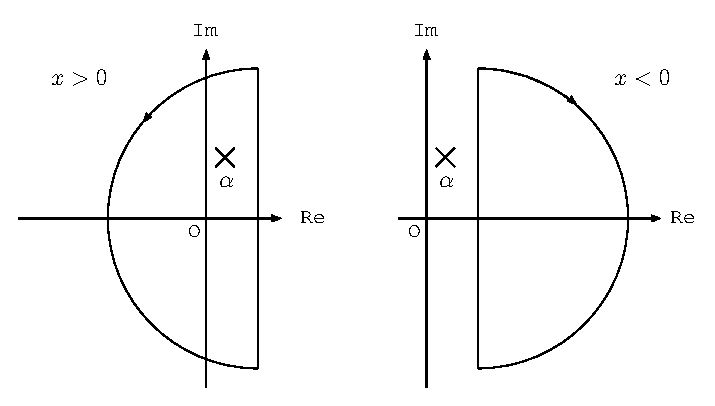
\includegraphics[width=.5\linewidth]{fig/laplace_int.eps}
  \end{center}
  \caption{
    ラプラス逆変換を行うための積分路。
    ジョルダンの補題により、$\e^{sx}$があるため、$x>0$の場合は
    左、$x<0$の場合は右を周る積分路を取らなくてはならない。
    このとき、ラプラス変換が存在する条件は、$s$の実部が
    すべての極の実部よりも大きいことなので、$x<0$の場合は
    必ず$0$となる。
  }
  \label{fig_laplace_int}
\end{figure}

\ans{30}{2}

前問と同様に$x<0$では$f(x) = 0$となるので、$x>0$の場合のみ考える。
\begin{eqnarray}
  f(x) &=& \frac{1}{2 \pi i} \int_C \diff z \frac{z \e^{zx}}{z^2+c^2}
\end{eqnarray}
ここで、特異点は$z = ic, -ic$の二つで、それぞれ一位の極である。
$z = ic$における留数は、
\begin{equation}
  \left. \frac{z \e^{zx}}{z+ic} \right|_{z = ic} = \frac{1}{2}\e^{icx}
\end{equation}
同様に$z = -ic$における留数は、
\begin{equation}
  \left. \frac{z \e^{zx}}{z-ic} \right|_{z = -ic} = \frac{1}{2}\e^{-icx}
\end{equation}
両方足せば、
\begin{equation}
  f(x) = \frac{\e^{icx}+\e^{-icx}}{2} = \cos cx
\end{equation}
を得る。

\ans{31}{1}
微分方程式全体をラプラス変換すると、$f(0)=f'(0)=0$より、
\begin{equation}
  (s^2 - 2s +1) \hat{y}(s) = \frac{1}{s^2}
\end{equation}
すなわち、
\begin{equation}
  \hat{y}(s) = \frac{1}{s^2 (s-1)^2}
\end{equation}
これを部分分数分解すると、
\begin{equation}
  \hat{y}(s) = \frac{-2}{s-1} + \frac{1}{(s-1)^2} + \frac{2}{s} + \frac{1}{s^2}
\end{equation}
ここで、それぞれ
\begin{eqnarray}
  {\cal L}[\e^x] &=& \frac{1}{s-1}\\
  {\cal L}[x\e^x] &=& \frac{1}{(s-1)^2}\\
  {\cal L}[1] &=& \frac{1}{s}\\
  {\cal L}[x] &=& \frac{1}{s^2}
\end{eqnarray}
であるから、
\begin{equation}
  f(x) = -2 \e^{x}+x\e^x+2+x
\end{equation}

微分方程式全体をラプラス変換すると、$f(0)=f'(0)=0$より、
\begin{equation}
  (s^2 + 2s +1) \hat{y}(s) = \frac{1}{s}
\end{equation}
すなわち、
\begin{equation}
  \hat{y}(s) = \frac{1}{s(s+1)^2}
\end{equation}
右辺を部分分数分解する。
やりかたを丁寧に解説すると、
\begin{equation}
  \frac{1}{s(s+1)^2} = \frac{a}{s} + \frac{b}{s+1} + \frac{c}{(s+1)^2}
\end{equation}
と分解できたとすると、両辺に$s$をかけてから$s=0$を代入すれば、
それは$a$である。
すなわち、
\begin{equation}
  a = \left. \frac{1}{(s+1)^2}\right|_{s=0} = 1
\end{equation}
同様に$(s+1)^2$を両辺にかけて$s=-1$を代入すれば、
\begin{equation}
  c = \left. \frac{1}{s}\right|_{s=-1} = -1
\end{equation}
$b$を求めるには、$(s+1)^2$を両辺にかけて微分してから$s=-1$を代入する。
よって、
\begin{equation}
  b = \left. \left(\frac{1}{s}\right)^2 \right|_{s=-1} = -1
\end{equation}
以上より、
\begin{equation}
  \hat{y}(s) =  \frac{1}{s} - \frac{1}{s+1} - \frac{1}{(s+1)^2}
\end{equation}
逆ラプラス変換すれば、
\begin{equation}
  y(x) =  1 - \e^{-x} - x\e^{-x}
\end{equation}
これは確かに$y(0)=y'(0) = 0$であり、
代入すると解になっている。


\subsection{解説}

\subsubsection{ラプラス変換}

フーリエ変換では、関数$f(x)$は無限区間$-\infty < x < \infty$で定義されていた。
変数を時間だと思えば、これは系に安定に存在する解について調べていることになる。
それに対し、電気回路にスイッチを入れたり、バネをはじいたりと、
それまで静的であった系になんらかの刺激を与えたときの応答を知りたい場合が
よくある。そのような過渡的な現象の解析に威力を発揮するのが
{\bf ラプラス変換 (Laplace transform)}である。
過渡的な現象は、微分方程式の初期値問題を解くことに帰着される。
ラプラス変換は、微分方程式の初期値問題を簡単に解く処方箋を与える。

\subsubsection{ラプラス変換とフーリエ変換}

ある関数$f(x)$に対して、次のような関数$g(x)$を考える。
\begin{equation}
  g(x) = \left\{
  \begin{array}{cc}
    0             & \qquad x<0      \\
    \e^{-ax} f(x) & \qquad x \geq 0
  \end{array}
  \right.
\end{equation}

ここで、$g(x)$をフーリエ変換すると、
\begin{eqnarray}
  {\cal F}[g(x)] &=& \int_{-\infty}^{\infty} \diff x g(x) \e^{-ikx}\\
  &=& \int_{0}^{\infty} \diff x \e^{-ax} f(x) \e^{-ikx}\\
  &=& \int_{0}^{\infty} \diff x f(x) \e^{-(a+ik)x}
\end{eqnarray}
ここで、$s = a+ik$とすると、
\begin{eqnarray}
  \int_{0}^{\infty} \diff x f(x) \e^{-(a+ik)x} &=& \int_{0}^{\infty} \diff x f(x) \e^{-sx}\\
  &=& {\cal L}[f(x)]
\end{eqnarray}
これは$f(x)$のラプラス変換に他ならない。
フーリエ変換不可能な関数でも、$a$を十分に大きく取れば$\e^{-ax} f(x)$の
積分が収束し、ラプラス変換が可能である場合がある。
すなわち、ラプラス変換とは、$\e^{-ax}$をかけて収束範囲を広げた
フーリエ変換と考えることができる。

さて、${\cal F}[g(x)]$をフーリエ逆変換しよう。
\begin{eqnarray}
  g(x) &=& \frac{1}{2\pi} \int_{-\infty}^{\infty} \diff k {\cal F}[g(x)] \e^{ikx}\\
  &=& \frac{1}{2\pi} \int_{-\infty}^{\infty} \diff k \hat{f}(s) \e^{ikx}
\end{eqnarray}
ここで、${\cal F}[g(x)] = \hat{f}(s)$であり、$x>0$であれば$g(x) = \e^{-ax} f(x)$であるから、
\begin{eqnarray}
  \e^{-ax} f(x) &=& \frac{1}{2\pi }  \int_{-\infty}^{\infty} \diff k \hat{f}(s) \e^{ikx}\\
  f(x) &=& \frac{1}{2\pi }  \int_{-\infty}^{\infty} \diff k \hat{f}(s) \e^{(a+ik)x}\\
\end{eqnarray}
$s = a + ik$と置くと、$\diff s = i \diff k$、
積分範囲が$a - \infty < s < a + \infty $となることから、
\begin{equation}
  f(x) = \frac{1}{2\pi i}  \int_{a-\infty}^{a+\infty} \diff s \hat{f}(s) \e^{sx}\\
\end{equation}
これは、ラプラス逆変換の定義である。

ここで$a$は 積分
\begin{equation}
  \int_0^{\infty} \e^{-ax} |f(x)| \diff x
\end{equation}
が収束するように選ばれたのであった。これは、$a$が$f(x)$のすべての極よりも
右側にくることを意味する\footnote{ここでは詳細は省略する。参考書を参照のこと}。
これによりラプラス逆変換が$x<0$の時に$f(x)=0$となる。
また、$s = a + ik$とおいたので、${\mathrm Re} s = a$である。
ラプラス変換において、$s$は一般に任意の複素数であるが、その実部は十分に
(ラプラス変換が収束するように)選ばれなければならない。

\subsubsection{非同次方程式とたたみ込み積分}

ラプラス変換は、線形非同次方程式を解くのに威力を発揮する(以下線形を略す)。
非同次方程式とは、次のような形の微分方程式である。
\begin{equation}
  u''(x) + u(x) = f(x) \label{eq_laplace_combo1}
\end{equation}

まず、$f(x)=\delta(x)$と置いた方程式を
\begin{equation}
  v''(x) + v(x) = \delta(x)
\end{equation}
と書こう。この解$v(x)$が得られたとすると、$u$を$v$で表すことができる。
まず、方程式全体をラプラス変換することで、
\begin{equation}
  {\cal L}[v] = \frac{1}{s^2+1} \label{eq_laplace_combo2}
\end{equation}
であることが分かる。
また、式(\ref{eq_laplace_combo1})をラプラス変換すれば、
\begin{equation}
  {\cal L}[u] = \frac{{\cal L}[f]}{s^2+1}\label{eq_laplace_combo3}
\end{equation}
である。式(\ref{eq_laplace_combo2})と式(\ref{eq_laplace_combo3})を見比べれば、
\begin{equation}
  {\cal L}[u] = {\cal L}[v] {\cal L}[f]
\end{equation}
たたみ込み積分のラプラス変換の性質から
${\cal L}[v] {\cal L}[f] = {\cal L}[v*f]$
であるから、
\begin{equation}
  u(x) = \int_0^{x} v(x-y)f(x)  \diff y
\end{equation}
と$u(x)$を$v(x)$で表すことができた。

すなわち、{\bf 同次方程式を解くことができれば、一般の
非同次方程式の解を得ることができる}。

デルタ関数とたたみ込み積分には物理的に重要な関係がある。
過渡的な現象にはたたみ込み積分が現れることが多い。
ある時刻$t=0$にデルタ関数的な刺激を与えたとき、
その出力(応答)が時刻$t$で$w(t)$となるような系を考える。
たとえば、LCR回路に瞬間的に電圧をかけたり、
ぴんと張った弦を弾いたりすると、系はしばらく振動して、
やがて落ち着いていくだろう。
このような応答を{\bf インパルス応答}と呼び、工学では特に重要な概念である。

デルタ関数に対する応答$w(t)$を用いて、任意の入力$f(x)$に対する
出力$h(t)$は
\begin{equation}
  h(t) = \int_0^t w(t-s) f(s) \diff s
\end{equation}
とたたみ込み積分の形で書くことができる。
この式は、時刻$s$での入力$f(s)$が、重み$w(t-s)$で
時刻$t$での出力$h(t)$に影響を与えているという意味を持っている。

%-----------------------------------------------------------------------
\section{おわりに}
%-----------------------------------------------------------------------

以上、物理で使われる数学を一通り学んだ。
かなり駆け足でやったので消化不良のところがあることだろう。
必要に応じて復習して欲しい。その際、教科書を読むだけでなく、
実際に手を動かしてみないと数学は身につかない。
物理で扱う方程式とその解には全て意味がある。
たとえば過渡的な現象であれば$t\rightarrow \infty$で$0$となるはずだろう。
波動方程式の解であれば、なんらかの波を表しているはずだから
周期的な運動を記述するだろう。
問題を解く際にはこのようなイメージを大事にして欲しい。

今回、電磁気学や流体力学で必要となるベクトル解析に
全く触れることができなかった。また、線形代数の扱いは不十分である。
必要であれば各自勉強して欲しい。

\end{document}


